%%% The main file. It contains definitions of basic parameters and includes all other parts.

%% Settings for single-side (simplex) printing
% Margins: left 40mm, right 25mm, top and bottom 25mm
% (but beware, LaTeX adds 1in implicitly)
\documentclass[12pt,a4paper]{report}
\setlength\textwidth{145mm}
\setlength\textheight{247mm}
\setlength\oddsidemargin{15mm}
\setlength\evensidemargin{15mm}
\setlength\topmargin{0mm}
\setlength\headsep{0mm}
\setlength\headheight{0mm}
% \openright makes the following text appear on a right-hand page
\let\openright=\clearpage

%% Settings for two-sided (duplex) printing
% \documentclass[12pt,a4paper,twoside,openright]{report}
% \setlength\textwidth{145mm}
% \setlength\textheight{247mm}
% \setlength\oddsidemargin{14.2mm}
% \setlength\evensidemargin{0mm}
% \setlength\topmargin{0mm}
% \setlength\headsep{0mm}
% \setlength\headheight{0mm}
% \let\openright=\cleardoublepage

%% Generate PDF/A-2u
\usepackage[a-2u]{pdfx}

%% Character encoding: usually latin2, cp1250 or utf8:
\usepackage[utf8]{inputenc}

%% Prefer Latin Modern fonts
\usepackage{lmodern}

%% Further useful packages (included in most LaTeX distributions)
\usepackage{amsmath}        % extensions for typesetting of math
\usepackage{amsfonts}       % math fonts
\usepackage{amsthm}         % theorems, definitions, etc.
\usepackage{bbding}         % various symbols (squares, asterisks, scissors, ...)
\usepackage{bm}             % boldface symbols (\bm)
\usepackage{graphicx}       % embedding of pictures
\usepackage{fancyvrb}       % improved verbatim environment
\usepackage{natbib}         % citation style AUTHOR (YEAR), or AUTHOR [NUMBER]
\usepackage[nottoc]{tocbibind} % makes sure that bibliography and the lists
			    % of figures/tables are included in the table
			    % of contents
\usepackage{dcolumn}        % improved alignment of table columns
\usepackage{booktabs}       % improved horizontal lines in tables
\usepackage{paralist}       % improved enumerate and itemize
\usepackage{xcolor}         % typesetting in color

\usepackage{times}
\usepackage{latexsym}
\usepackage{tipa}
\usepackage[normalem]{ulem} % sout
\usepackage[noabbrev,capitalize]{cleveref}
\usepackage{tikz}
\usetikzlibrary{positioning,shapes,arrows,calc,decorations.pathmorphing}
\usepackage{textcomp}
\usepackage{makecell}
\usepackage{enumitem}
\usepackage{pgfplots}
\usepackage{tikzscale}
\usepackage{microtype}
\usepackage{rotating}
\usepackage{pdflscape}
\usepackage{multirow}


%%% Basic information on the thesis

% Thesis title in English (exactly as in the formal assignment)
\def\ThesisTitle{Spoken Language Translation via Phoneme Representation of the Source Language}

% Author of the thesis
\def\ThesisAuthor{Peter Polák}

% Year when the thesis is submitted
\def\YearSubmitted{2020}

% Name of the department or institute, where the work was officially assigned
% (according to the Organizational Structure of MFF UK in English,
% or a full name of a department outside MFF)
\def\Department{Institute of Formal and Applied Linguistics}

% Is it a department (katedra), or an institute (ústav)?
\def\DeptType{Institute}

% Thesis supervisor: name, surname and titles
\def\Supervisor{doc. RNDr. Ondřej Bojar, Ph.D.}

% Supervisor's department (again according to Organizational structure of MFF)
\def\SupervisorsDepartment{Institute of Formal and Applied Linguistics}

% Study programme and specialization
\def\StudyProgramme{Computer Science}
\def\StudyBranch{Artificial Intelligence}

% An optional dedication: you can thank whomever you wish (your supervisor,
% consultant, a person who lent the software, etc.)
\def\Dedication{%
Dedication.
}

% Abstract (recommended length around 80-200 words; this is not a copy of your thesis assignment!)
\def\Abstract{%
Abstract.
}

% 3 to 5 keywords (recommended), each enclosed in curly braces
\def\Keywords{%
{key} {words}
}

%% The hyperref package for clickable links in PDF and also for storing
%% metadata to PDF (including the table of contents).
%% Most settings are pre-set by the pdfx package.
\hypersetup{unicode}
\hypersetup{breaklinks=true}

% Definitions of macros (see description inside)
%%% This file contains definitions of various useful macros and environments %%%
%%% Please add more macros here instead of cluttering other files with them. %%%

%%% Minor tweaks of style

% These macros employ a little dirty trick to convince LaTeX to typeset
% chapter headings sanely, without lots of empty space above them.
% Feel free to ignore.
\makeatletter
\def\@makechapterhead#1{
  {\parindent \z@ \raggedright \normalfont
   \Huge\bfseries \thechapter. #1
   \par\nobreak
   \vskip 20\p@
}}
\def\@makeschapterhead#1{
  {\parindent \z@ \raggedright \normalfont
   \Huge\bfseries #1
   \par\nobreak
   \vskip 20\p@
}}
\makeatother

% This macro defines a chapter, which is not numbered, but is included
% in the table of contents.
\def\chapwithtoc#1{
\chapter*{#1}
\addcontentsline{toc}{chapter}{#1}
}

% Draw black "slugs" whenever a line overflows, so that we can spot it easily.
\overfullrule=1mm

%%% Macros for definitions, theorems, claims, examples, ... (requires amsthm package)

\theoremstyle{plain}
\newtheorem{thm}{Theorem}
\newtheorem{lemma}[thm]{Lemma}
\newtheorem{claim}[thm]{Claim}

\theoremstyle{plain}
\newtheorem{defn}{Definition}

\theoremstyle{remark}
\newtheorem*{cor}{Corollary}
\newtheorem*{rem}{Remark}
\newtheorem*{example}{Example}

%%% An environment for proofs

\newenvironment{myproof}{
  \par\medskip\noindent
  \textit{Proof}.
}{
\newline
\rightline{$\qedsymbol$}
}

%%% An environment for typesetting of program code and input/output
%%% of programs. (Requires the fancyvrb package -- fancy verbatim.)

\DefineVerbatimEnvironment{code}{Verbatim}{fontsize=\small, frame=single}

%%% The field of all real and natural numbers
\newcommand{\R}{\mathbb{R}}
\newcommand{\N}{\mathbb{N}}

%%% Useful operators for statistics and probability
\DeclareMathOperator{\pr}{\textsf{P}}
\DeclareMathOperator{\E}{\textsf{E}\,}
\DeclareMathOperator{\var}{\textrm{var}}
\DeclareMathOperator{\sd}{\textrm{sd}}

%%% Transposition of a vector/matrix
\newcommand{\T}[1]{#1^\top}

%%% Various math goodies
\newcommand{\goto}{\rightarrow}
\newcommand{\gotop}{\stackrel{P}{\longrightarrow}}
\newcommand{\maon}[1]{o(n^{#1})}
\newcommand{\abs}[1]{\left|{#1}\right|}
\newcommand{\dint}{\int_0^\tau\!\!\int_0^\tau}
\newcommand{\isqr}[1]{\frac{1}{\sqrt{#1}}}

%%% Various table goodies
\newcommand{\pulrad}[1]{\raisebox{1.5ex}[0pt]{#1}}
\newcommand{\mc}[1]{\multicolumn{1}{c}{#1}}


\def\XXX#1{{\textcolor{red}{XXX #1}}}


% Definition of blocks:
\tikzset{%
	block/.style    = {draw,  rectangle, minimum height = 2.7em,
		minimum width = 3em}
}

\renewcommand{\UrlFont}{\ttfamily\small}

% This is not strictly necessary, and may be commented out,
% but it will improve the layout of the manuscript,
% and will typically save some space.

%\aclfinalcopy % Uncomment this line for the final submission
%\def\aclpaperid{***} %  Enter the acl Paper ID here

%\setlength\titlebox{5cm}
% You can expand the titlebox if you need extra space
% to show all the authors. Please do not make the titlebox
% smaller than 5cm (the original size); we will check this
% in the camera-ready version and ask you to change it back.

\newcommand\BibTeX{B\textsc{ib}\TeX}


\def\XXX#1{{\textcolor{red}{XXX #1}}}
\def\repl#1#2{{\textcolor{red}{\sout{#1}}\textcolor{blue}{#2}}}
\def\parcite#1{\citep{#1}} % (Smith, 2012)
\def\perscite#1{\citet{#1}} % Smith (2012)
\def\inparcite#1{\citealp{#1}} % should be Smith, 2012

\def\footurl#1{\footnote{\url{#1}}}

\newcommand\litem[1]{\item{\bfseries #1}}

% Title page and various mandatory informational pages
\begin{document}
%%% Title page of the thesis and other mandatory pages

%%% Title page of the thesis

\pagestyle{empty}
\hypersetup{pageanchor=false}
\begin{center}

\centerline{\mbox{
\includegraphics[width=166mm]{img/logo-en.pdf}}}

\vspace{-8mm}
\vfill

{\bf\Large MASTER THESIS}

\vfill

{\LARGE\ThesisAuthor}

\vspace{15mm}

{\LARGE\bfseries\ThesisTitle}

\vfill

\Department

\vfill

{
\centerline{\vbox{\halign{\hbox to 0.45\hsize{\hfil #}&\hskip 0.5em\parbox[t]{0.45\hsize}{\raggedright #}\cr
Supervisor of the master thesis:&\Supervisor \cr
\noalign{\vspace{2mm}}
Study programme:&\StudyProgramme \cr
\noalign{\vspace{2mm}}
Study branch:&\StudyBranch \cr
}}}}

\vfill

% Zde doplňte rok
Prague \YearSubmitted

\end{center}

\newpage

%%% Here should be a bound sheet included -- a signed copy of the "master
%%% thesis assignment". This assignment is NOT a part of the electronic
%%% version of the thesis. DO NOT SCAN.
This is not a~part of the electronic version of the thesis, do not scan!

%%% A page with a solemn declaration to the master thesis

\openright
\hypersetup{pageanchor=true}
\pagestyle{plain}
\pagenumbering{roman}
\vglue 0pt plus 1fill

\noindent
I declare that I carried out this master thesis independently, and only with the cited
sources, literature and other professional sources. It has not been used to obtain another
or the same degree.

\medskip\noindent
I understand that my work relates to the rights and obligations under the Act No.~121/2000 Sb.,
the Copyright Act, as amended, in particular the fact that the Charles
University has the right to conclude a license agreement on the use of this
work as a school work pursuant to Section 60 subsection 1 of the Copyright~Act.

\vspace{10mm}

\hbox{\hbox to 0.5\hsize{%
In \hbox to 6em{\dotfill} date \hbox to 6em{\dotfill}
\hss}\hbox to 0.5\hsize{\dotfill\quad}}
\smallskip
\hbox{\hbox to 0.5\hsize{}\hbox to 0.5\hsize{\hfil Author's signature\hfil}}

\vspace{20mm}
\newpage

%%% Dedication

\openright

\noindent
\Dedication

\newpage

%%% Mandatory information page of the thesis

\openright

\vbox to 0.5\vsize{
\setlength\parindent{0mm}
\setlength\parskip{5mm}

Title:
\ThesisTitle

Author:
\ThesisAuthor

\DeptType:
\Department

Supervisor:
\Supervisor, \SupervisorsDepartment

Abstract:
\Abstract

Keywords:
\Keywords

\vss}

\newpage

\openright
\pagestyle{plain}
\pagenumbering{arabic}
\setcounter{page}{1}

%%% A page with automatically generated table of contents of the master thesis

\tableofcontents

%%% Each chapter is kept in a separate file

\chapter*{Introduction}
\addcontentsline{toc}{chapter}{Introduction}

\section*{Work organization}
We settled on a less traditional strategy for the organization of this work: we serve every chapter as a standalone small paper. Notably, each chapter includes a section about related work devoted to the chapter's subject. We review mutual related work in \cref{chap:theory} (such as neural network architectures or corpora).

Chapters progressively deal with problematic starting with Automatic Speech Recognition in \cref{chapter:asr}, further enhancing ASR in \cref{chap:enhanced_asr}, continuing with Spoken Language Translation in \cref{chap:slt}. Adaptation to speaker is described in \cref{chap:adaptation}. We also deal with ``bringing our work to life'' in \cref{chap:onlinezation}. Finally, we conclude the work in \cref{chap:conclusion}.


\chapter{Tasks, architectures, and data sets}
\label{chap:theory}
In this chapter, we give a brief overview of the theoretical foundations necessitated for this thesis. First, we define the main tasks that are part of the solution. Moreover, we describe the utilized neural network architectures. Lastly, we describe used data sets and introduce evaluation metrics.

\section{Automatic Speech Recognition}

Automatic Speech Recognition (ASR) is one of the most popular tasks in NLP, and without a doubt, it is one of the most important ones. With ever-growing technology that becomes more and more integrated with our day-to-day life, it is clear that ASR will take an essential role in this process.

In this section, we first briefly examine the history and then describe the most popular contemporaneous approaches for ASR.

\subsection{Brief history}

The first attempts for ASR systems stem from the 1950s. At that time, researchers focused their interest on acoustics-phonetics, which describes phonetic elements of speech, including phonemes \parcite{juang2005automatic}. The first ASR system worked with syllables, vowels, and phonemes. An example can be taken spoken digit recognizer from Bell laboratories. Their system estimated formant frequencies (as a vowel is pronounced, vocal tract sounds with natural modes of resonance called formant) of vowel regions of an isolated digit. 

A big leap in ASR systems was the introduction and popularization of Hidden Markov models (HMMs) in the 1980s. HMMs caused architecture to shift from pattern recognition to statistical modeling. The success of HMM-based ASR systems continues even today in the form of hybrid models consisting of HMMs and either Gaussian Mixture Models (GMMs) or Artificial Neural Networks (ANNs).

In the last few years, deep neural networks gained much popularity. In many tasks, ranging from image processing to natural language processing, DNNs outperformed other known methods. Besides their performance, they tend to require less expertise and engineering skills for a particular task than other methods. This makes them available for researchers in many areas. DNNs are becoming a standard in ASR currently, but the first attempts were already made briefly after the introduction of the backpropagation algorithm \parcite{rumelhart1986learning}. They were used for recognition of phonemes \parcite{waibel1989phoneme} or few words \parcite{lubensky1988learning}. Further important milestones for ASR in the 2010s were recurrent neural networks and attention (applied, for example, in \perscite{chorowski2014end}) in the 2010s.

\subsection{Models}
In this section, we introduce contemporary models utilized for ASR. There are two such approaches: (1) HMM-based models, (2) End-to-End neural models.

\subsubsection{HMM-based models}
HMMs (Hidden Markov Models) are probably the most used technique in ASR \parcite{padmanabhan2015machine}. HMMs are in the ASR context used with either GMMs (Gaussian Mixture Models)  or ANNs (Artificial Neural Networks).  Practitioners often refer to the HMM-based models as a hybrid.

A typical pipeline of an HMM-based model works as follows: the input is first pre-processed and converted to features, typically the MFCCs (see \cref{mfcc}). These featured are further passed to the estimator. Common, estimated units in HMM-based pipelines are phones. The decoder employs \emph{acoustic model}, \emph{dictionary} and \emph{language model} to decode the speech. The acoustic model estimates the probability of the acoustic sequence given word sequence. ANNs or GMMs represents the acoustic model. Dictionary maps phone sequences to words. Finally, the language model estimates the apriori probability of word sequence, independent of observed sound. Usual are $n$-gram language models. 

\subsubsection{End-to-End models}
Opposed to the HMM-based models are End-to-End ASR pipelines. The common trait for these models is their ability to produce the final, human-readable text given acoustic features using one end-to-end deep neural network. Recent advancements (for example, \perscite{amodei2016deep,Li2019}) in the ASR field clearly show the future direction towards this kind of ASR. The advantage of the E2E model is that they require less engineering than HMM models. Open problem remains the higher requirement of training data.

The input of the model are MFCC features extracted from speech data. E2E model then outputs probabilities of graphemes at each time step employing CTC loss. Applications extend conventional beam search with language model (again, $n$-gram LM is used) that re-scores the beams during the decoding. The use of LM in the beam search further enhances the transcription quality.

\section{\XXX{Spoken Language Translation or Speech translation}}
Spoken Language Translation is another NLP task dealing with the translation of the speech. \XXX{In literature, the SLT task describes translation into a target language text. Commonly, SLT can also be a speech-to-speech translation.} Traditional layout of speech translation, before the emergence of end-to-end systems, consisting of a speech recognition unit followed by machine translation. With the upraise of deep learning, E2E frameworks that do not need intermediate transcription step are gaining popularity \parcite{berard2016listen,berard2018end,jia2019leveraging}.

Direct comparison of both methods seems inconclusive \parcite{sperber2019attention}. Also, the actual tasks of E2E and cascaded SLT differ: E2E SLT must be trained on E2E corpora, while the cascading can be trained on independent corpora for ASR and MT. This makes the latter suitable in cases where is no corpus for given language pair available (which is mostly the case). On the other hand, cascading speech recognition and machine translation for SLT could introduce errors in source language transcription that might be further propagated to final translation.

\section{Models/architectures}
In this section, we introduce neural network models/architectures we engage in our work. The first two models, Jasper and QuartzNet, are used as acoustic models. Finally, we present the Transformer, which serves as a translation and correction model.

\subsection{Jasper}

Jasper \parcite{Li2019} is a family of end-to-end, deep convolutional neural network ASR architectures. We incorporate the architecture in our ASR and SLT pipelines.

\subsubsection{Architecture Overview}
The input of the model are Mel Frequency Cepstrum Coefficients (see \cref{mfcc}) obtained from 20 ms frames with 10 ms stride. We use 64 features. The model outputs probability over given vocabulary for every processed frame. In our pipeline, the vocabulary is IPA phonemes.

Input is passed through one pre-processing layer, followed by the central part of the network. Finally, tree post-processing layers are applied. The central part of the model consists of so-called ``blocks''.

Jasper model consists of $B$ blocks and $R$ sub-blocks. Jasper authors introduce a naming convention where such model is described as ``Jasper $B$x$R$''. In our work, we use Jasper 10x5.

Sub-blocks applying operations as follows: 1D convolution, ReLU activation, and dropout. All sub-blocks of a block have the same number of output channels. 

The input of a block is connected to the last sub-block via residual connection. Because the number of channels differs, 1x1 convolution is applied to account this. After this projection, batch normalization is applied. The output is then added to the output of the batch normalization layer in the last sub-block. Afterward, activation function and dropout are used, producing the output of the current block.

Further, Jasper's authors observed that models deeper than Jasper 5x3 require residual connections to converge. Residual connections inspired by DenseNet \parcite{huang2017densely} and DenseRNet \parcite{tang2018acoustic} are employed.

Schema of the Jasper with residual connections is pictured in \cref{fig:jasper_dr}. The biggest used configuration for English (graphemes) has 333 million parameters.

\begin{figure}[h]
	\centering
	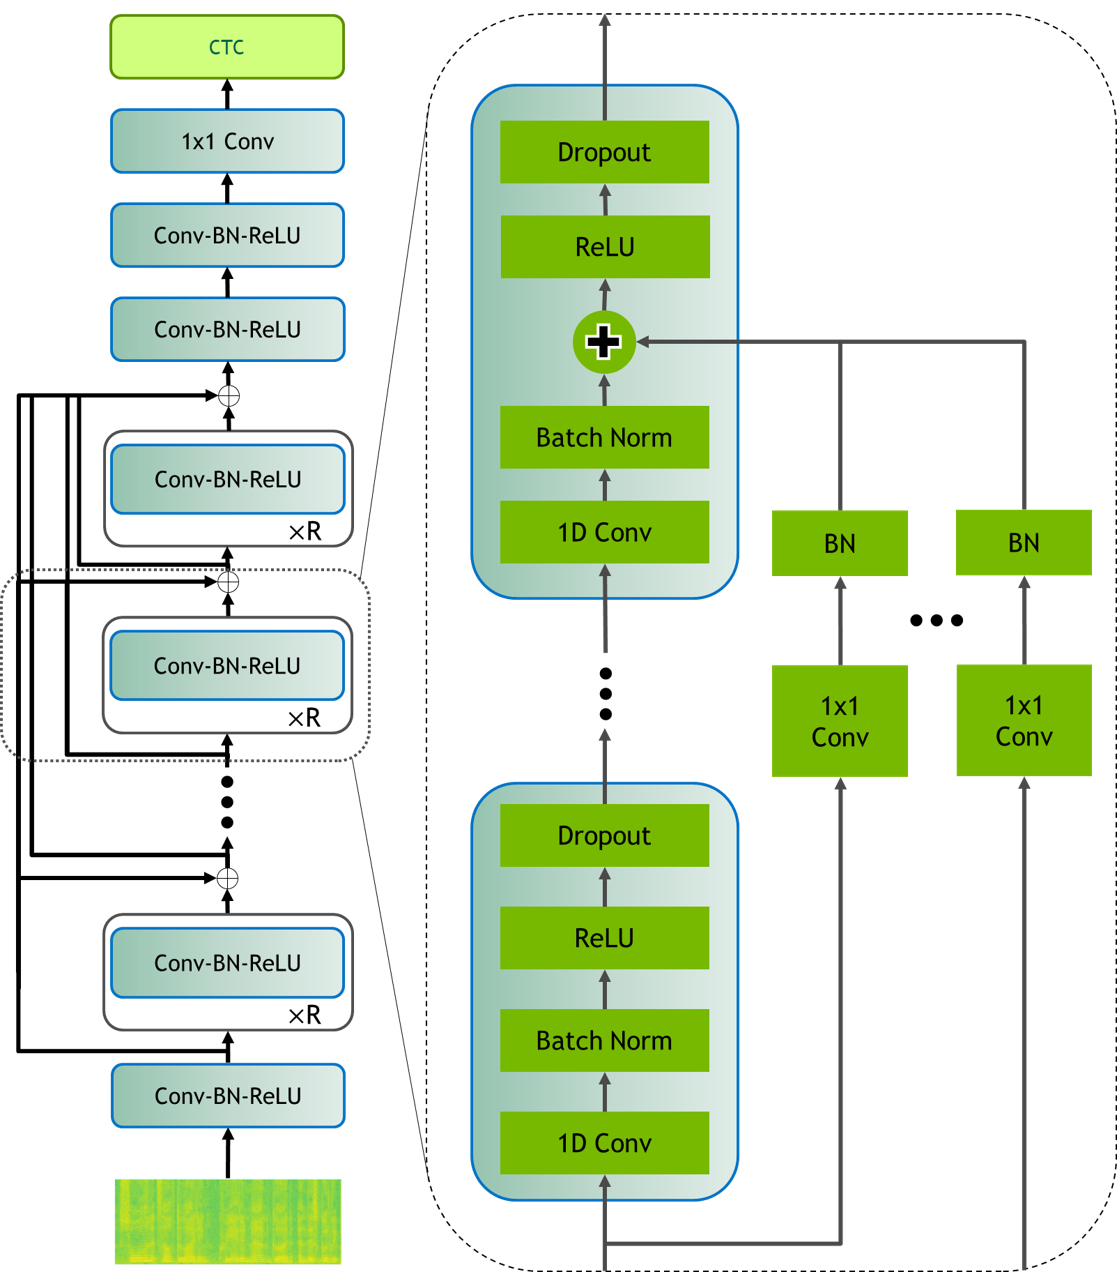
\includegraphics[scale=0.7]{img/JasperVerticalDR4.png}
	\caption{Jasper Dense Residual, taken from \perscite{li2019jasper}.}
	\label{fig:jasper_dr}
\end{figure}

\subsection{QuartzNet}

QuartzNet \parcite{kriman2019quartznet} is another end-to-end ASR architecture used in our work. QuartzNet is a convolutional neural network based on Jasper \parcite{Li2019} architecture having a fraction of parameters (18.9 million versus 333 million) while still achieving near state-of-the-art accuracy.

Same as the Jasper model, the network's input is 64 MFCC features computed from windows of length 20 ms and overlap 10 ms. The network outputs probability over the given alphabet for each time frame. For training is used CTC loss and for decoding beam search.

The main difference between the model and Jasper is the application of 1D time-channel separable convolutions.  Such convolutions can be separated into 1D depthwise convolutional layers with kernel $K$ and a pointwise convolution operating on each time frame independently. Because of this separation, the model has fewer parameters and can even have $3 \times$ larger kernel than the bigger Jasper model.

A further reduction of weights can be achieved by using grouped pointwise convolution instead of the pointwise convolution layer (see  \cref{fig:quartz_arch_groups}). When using four groups, the number of parameters is halved (for QuartzNet-15x5 from 18.9M to 8.7M) with slightly worse performance (WER 3.98 increases to 4.29 for LibriSpeech dev clean and 11.58 increases to 13.48).

As the first described weights reduction is sufficient for our purposes, we work with QuertzNet without the grouped pointwise convolution.

\begin{figure}[h]
	\centering
	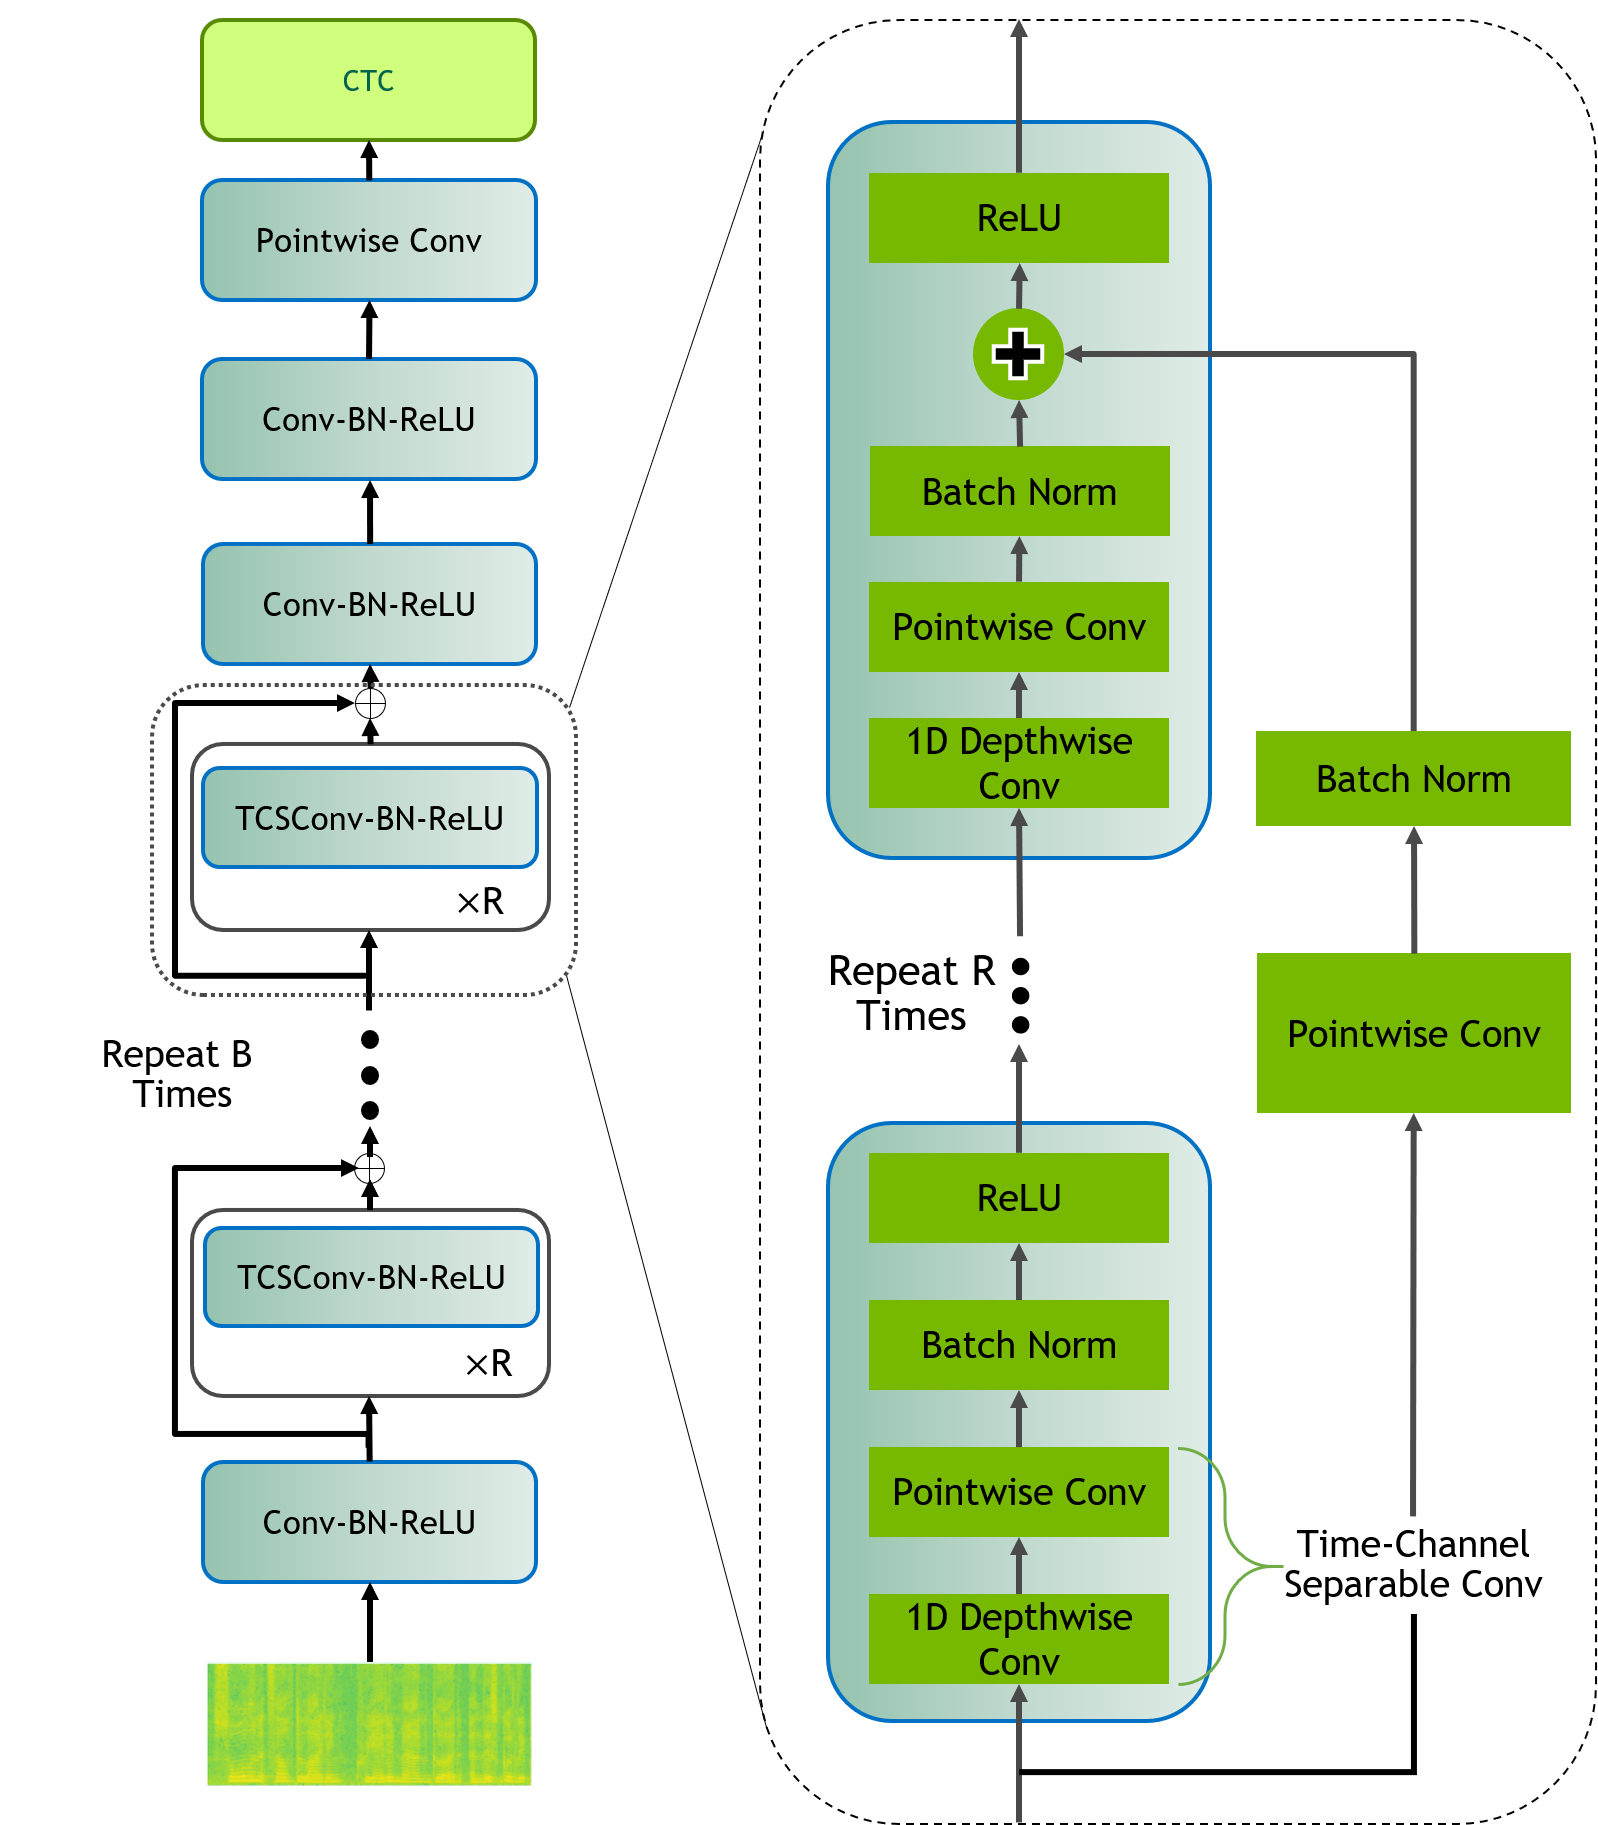
\includegraphics[width=\linewidth]{img/QuartzNet_v2.png}
	\caption{QuartzNet BxR architecture. Taken from \perscite{kriman2019quartznet}.}
	\label{fig:quartz_arch}
\end{figure}

\begin{figure}[h]
	\centering
	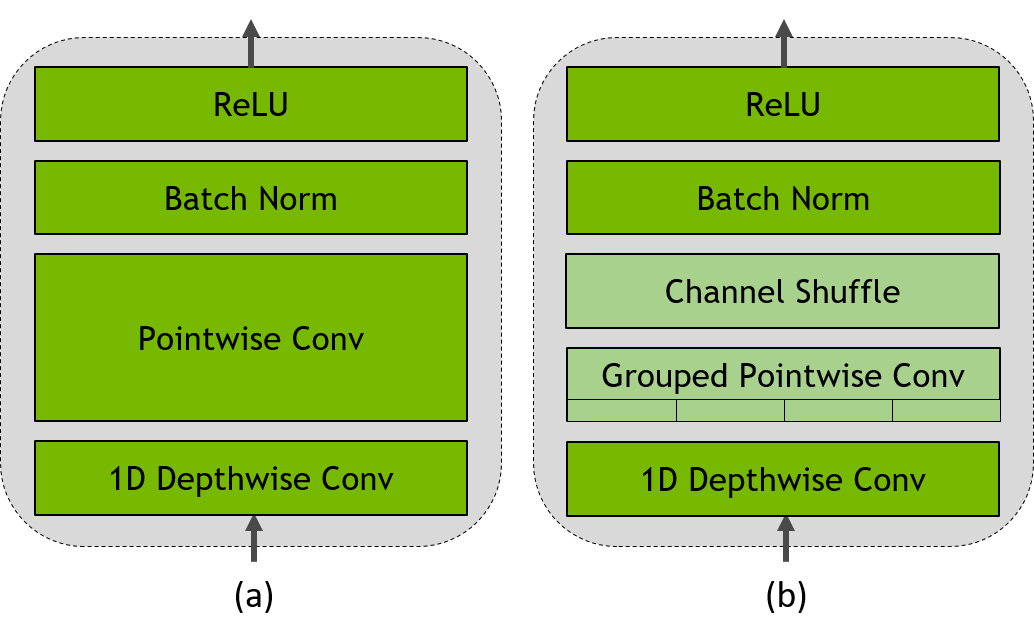
\includegraphics[width=0.8\linewidth]{img/QuartzNet_Grouped_v2.png}
	\caption{(a) Time-channel separable 1D convolutional module (b) Time-channel separable 1D convolutional module with groups and shuffle. Taken from \perscite{kriman2019quartznet}.}
	\label{fig:quartz_arch_groups}
\end{figure}


\subsection{Transformer}
Transformer \parcite{vaswani2017attention} has become a very good established architecture in Neural Machine Translation \parcite{bojar2018proceedings,barrault2019findings}. The main idea behind the architecture is to get rid of recurrence and convolutions and rather base the model solely on attention. As the attention mechanism is implemented as matrix multiplications, contemporary GPUs can better parallelize the computations leading to faster training.

A Transformer model is composed of encoder and decoder (see \cref{fig:transformer}). Both encoder and decoder are stacked identical layers. Encoder layer has two sub-layers: a multi-head self-attention layer and a fully connected feed-forward network. Decoder layer has extra multi-head attention sub-layer, which performs attention over the output of the encoder. This additional layer is between the self-attention and the feed-forward layers. Self-attention in the decoder is modified so that the auto-regressive property holds, i.e., the encoder cannot look to the right side (``future'').

The advantage of self-attention is that it can access arbitrary position in a constant number of sequentially executed operations while recurrent networks need $O(n)$ sequentially executed operations. If the sequence length is less than the representation dimension, which is often the case, the total computational complexity is lower than of the recurrent models. Another advantage presented by the authors is that self-attention leads to better interpretable models. They claim the individual attention heads seem to learn some specific functions that may be related to the syntactic and semantic structure of a sentence.

We employ this model in our enhanced ASR pipeline as a correction and language model and as a translation model in our SLT pipeline. 

\begin{figure}[h]
	\centering
	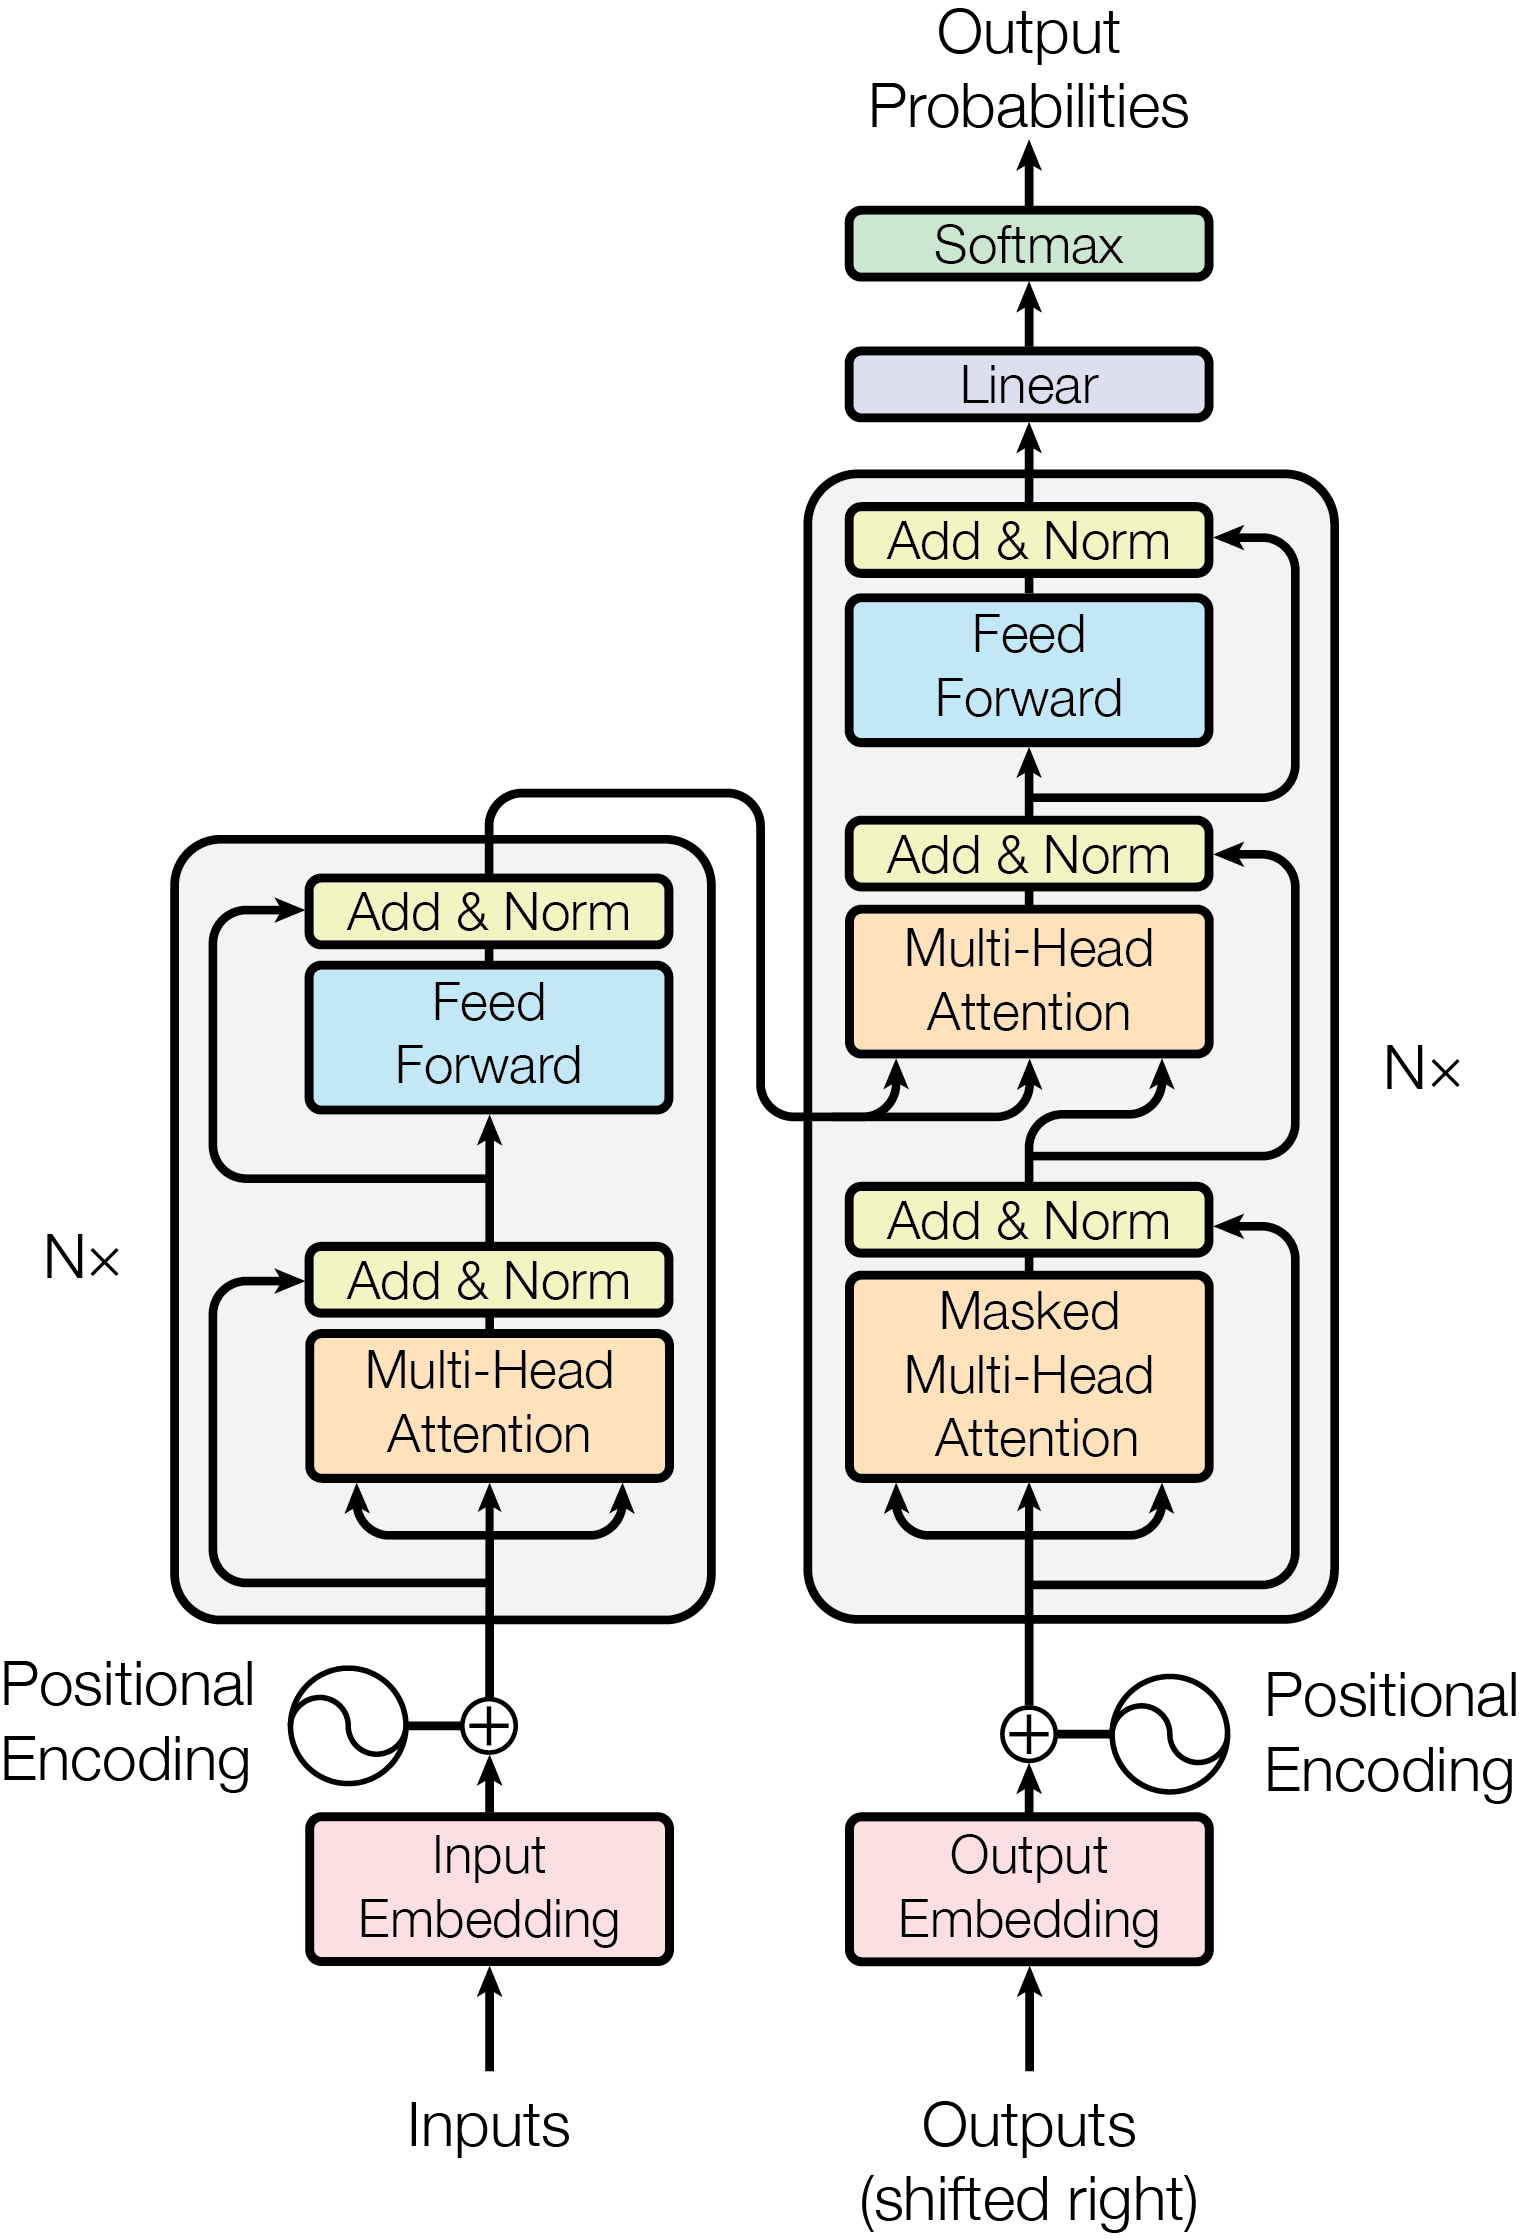
\includegraphics[width=0.8\linewidth]{img/ModalNet-21.png}
	\caption{Transformer model architecture with detailed encoder (left) and decoder (right). Taken from \perscite{vaswani2017attention}}
	\label{fig:transformer}
\end{figure}

\section{Data representation}
This section introduces to the reader the data representations. The way how we encode and feed the neural network can significantly influence performance. In this work, we transcribe recordings, i.e., we work with voice and text data. First, we introduce MFCC --- the voice presentation, and then we discuss text encoding.

\subsection{MFCC}
\label{mfcc}
Mel frequency cepstral coefficiets (MFCC) is the most commonly used representation of speech for ASR and SLT. 
This method exploits the way how the human auditory system perceives voice. Filter in the MFCC pipeline is linearly spaced for frequencies up to 1000 Hz and logarithmically above. 

MFCC pipeline as described in \perscite{muda2010voice} and \perscite{kamath2019deep}:

\begin{enumerate}
	\litem{Pre-emphasis} Application of filter that emphasises higher frequencies:
	
	\begin{equation}
	Y[n] = X[n] - \alpha X[n-1]
	\end{equation}.
	
	This filter makes the signal less dependent on strong signals from previous time steps.
	
	\litem{Framing} Raw audio is segmented into small windows. Signal in small windows can be then treated as stationary. Typically, the length of the window is about 20 ms, and windows have an overlap of 10 ms.
	
	\litem{Windowing} To avoid potential abrupt changes caused by framing windowing is applied. Windowing is a multiplication of samples in a window with a scaling function. Most commonly used in ASR is Hann and Hamming windowing:
	\begin{equation}
	w(n) = \sin^2{\left( \frac{\pi n}{N - 1} \right)}
	\end{equation}
	\begin{equation}
	w(n) = 0.54 - 0.46 \cos{\left(\frac{2\pi n}{N - 1}\right)}
	\end{equation}
	where $N$ is window length and $0 \leq n \leq N - 1$.
	
	\litem{Fast Fourier Transform} FFT converts one-dimensional signal from time to frequency domain.
	
	\litem{Mel Filter Bank}
	The Mel Filter Bank is a set of filters that mimic the human auditory system. Usually, 40 filters are used. Each filter is of a triangular shape. These are used to compute a weighted sum of spectral filter components approximating the Mel scale.
	Each filter output is then the sum of its filtered spectral components. 
	
	\litem{Discrete Cosine Transform} This process converts the log Mel spectrum into a time domain. The result is called the Mel Frequency Cepstrum Coefficient (the MFCC), and the set of coefficients is called acoustic vectors.
\end{enumerate}

An example of a mel-spectrogram is in the \cref{fig:mel}.

\begin{figure}[h]
	\centering
	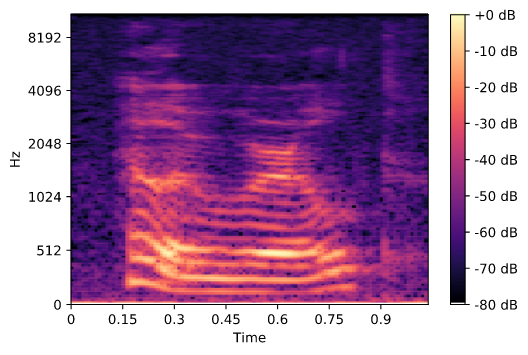
\includegraphics[width=0.8\linewidth]{img/mel.png}
	\caption{Mel spectogram of ``Hello World!''.}
	\label{fig:mel}
\end{figure}

\subsection{Text representation in NMT}

There are many approaches to text representation in NMT. Each of these representations has its advantages and drawbacks. We differentiate the following representations:

\begin{itemize}
	\item character,
	\item word,
	\item sub-word level representation.
\end{itemize}

The first one is a very simple and straightforward approach. Character representation permits one to encode any word (written in given characters). Its downside is that it produces longer sequences compared with other methods. Less output classes lead to the reduction of computational complexity. However, the model needs to attend more positions, which substantially increases time complexity during decoding.

Word level representation, on the other hand, produces shorted sequences. It may be better in some applications as the encoded string is shorter compared with the character-level approach. Generally, though, neural machine translation is an open-vocabulary problem. Word-level representation is undesirable, as it cannot handle unknown words. Several techniques have been proposed, such as NMT with post-processing step \parcite{luong2014addressing,luong2016achieving}.

The most versatile method seems to be a sub-word representation. It addresses both problems, as it produces shorter sequences compared, and is also capable of handling unknown and rare words. The number of contemporary NMTs that use sub-word level representation demonstrates its utility. The most prominent sub-word level tokenizers are BPEs \parcite{sennrich2016neural} and subword regularization \perscite{kudo2018subword}. Both methods are based on similar ideas --- they produce more compact text representations. The former is based on the ``merge'' operation that joins the most frequent character sequences together, while the latter is based on unigram language model. A particular benefit of the subword regularization is that it is also able to produce different segmentation.

In our work, we use BPE implementation YouTokenToMe\footnote{\url{https://github.com/VKCOM/YouTokenToMe}}. We chosen this particular implementation as it supports multithreading is considerably faster than other implementations and has Python and command-line interface. Further, it comes with BPE-dropout \parcite{provilkov2019bpe}. BPE-dropout is an enhancement of traditional BPE, which addresses the deterministic nature of the method. BPE-dropout randomly drops some merges from the BPE merge table, which results in different segmentation. Introducing a noise to the data helps to regularize an NMT model training.

\subsubsection{Byte Pair Encoding}
We would like to point out inconsistency of reporting BPE size in literature. Some authors use terms ``\textit{BPE size}'' and ``\textit{number of merge operations}'' as synonyms, although the actual \textit{BPE size} equals \textit{number of merge operations} plus \textit{characters}. In this work, we use term ``\textit{BPE size}'' as absolute vocabulary size --- including characters. 

\section{Data sets}
We dedicate this section to data sets used for the training of models in our work. First, we introduce speech corpora LibriSpeech and Common Voice, and then we introduce translation corpus CzEng.

\subsection{LibriSpeech}
LibriSpeech \parcite{panayotov2015librispeech} is a large corpus of read English speech. The corpus contains 1000 hours of transcribed speech based on audiobooks from project VoxForge\footnote{\url{http://www.voxforge.org/}}.

The data set is structured into three parts that have approximately 100, 360, and 500 hours. Using a trained model on the Wall Street Journal corpus \parcite{paul1992design}, authors divided the speakers by WER into two pools: ``clean'' and ``other''. From the ``clean'' pool, 20 male and female speakers were randomly selected to development and test sets. The rest was assigned to 100 and 360 hours of ``clean'' sets. For the ``other'' pool (500 hours), authors selected more challenging data for development and test sets.

\subsection{Common Voice}

Common Voice \perscite{ardila2019common} is a multi-lingual, crowdfunded speech corpus. At the time of the writing, 29 languages were available. English data set contained 1118 hours of validated, transcribed recordings. Unfortunately, the Czech data set was not available.

All utterances are collected and validated by volunteers. The data collection runs solely online through a web form. Speech utterances are stored in MPEG-3 format with a 48 kHz sampling rate. After at least two out of three volunteers up-votes an utterance, it is considered to be valid.

The number of clips is divided among the three datasets according to statistical power analyses.  Given the total number of validated clips in a language, the number of clips in the test set is equal to the amount needed to achieve a confidence level of 99\% with a margin of error of 1\% relative to the number of clips in the training set.  The same is true of the development set.

\subsection{Large Corpus of Czech Parliament Plenary Hearings}
Large Corpus of Czech Parliament Plenary Hearings \perscite{dataset} is a corpus of Czech transcribed speech. In our work, we use this dataset for the training of Czech ASR. The corpus has approximately 400 hours. As usual, the dataset contains training, evaluation, and test sets with no overlap. Training and development sets may have some common speakers. The test set should have no speaker overlap with the rest of the corpus.

A notable contrast with other speech corpora is the segmentation. The authors segmented the recordings into short utterances (the longest one has 44s), disregarding the sentences.

\subsection{CzEng 1.7}
Czeng 1.7 is a Czech-English parallel corpus containing about half a billion words. Czeng 1.7 is a filtered version of Czeng 1.6 \parcite{bojar2016czeng}. The advantage of the Czeng corpus is its rich origins such as subtitles, EU legislation, fiction, web pages, technical documents, or medical data. 

\subsubsection{Filtered CzEng}
\label{filtered_czeng}
For our purposes, we distilled out all sentence pairs that ``probably'' do not occur in spoken language. We assume the following: characters, numbers, apostrophe, punctuation, currency sign, dash, and quotation marks on the English side mark the sentence pair as a ``probable'' spoken utterance. Moreover, we filtered out too long and too short sentences (sentences must have at least two characters, at most 511 characters).

We intend to filter out sentences as for example \\

\begin{minipage}{0.95\linewidth}
	\small\emph{E-006961/11 (PL) Marek Henryk Migalski (ECR) to the Commission (15 July 2011)}\\
\end{minipage}


Such utterances do not have straightforward pronunciation, could break \texttt{phone\-mi\-zer}, and could degrade the transcript and translation quality.

\section{Error Metrics}
In this work, we use two error metrics, one for measuring the quality of speech recognition systems --- word error rate (WER) --- and a metric for evaluation of spoken language translation --- BLEU.

\subsection{Word Error Rate}
Word error rate is one of the most commonly used metrics. This metric measures edit distance (insertions, deletions, and substitutions) between target and hypothesis:

\begin{equation}
WER = 100 \times \frac{I + D + S}{N}
\end{equation}

where

\begin{itemize}
	\item $I$ is number of insertions,
	\item $D$ is number of deletions,
	\item $S$ is number of substitutions,
	\item $N$ is number of words in target.
\end{itemize}

Similarly is defined character error rate where, instead of words, are characters considered.

\subsection{BLEU}
For the evaluation of translation tasks, we use BLEU (Bilingual Evaluation Understudy) score introduced by \perscite{papineni2002bleu}. This metric assigns scores in the interval $[0,1]$, where 1 is the perfect score. The method counts occurrences of matching n-grams in candidate and reference (there can be more than one reference translations). It computes a modified n-gram precision (number of occurrences of an n-gram in candidate sentence must not exceed the maximum number of occurrences in any reference, otherwise is clipped) and does a weighted geometric mean. In addition to the implicit penalization of length, the metric introduces the brevity penalty.

Usage of this metric used to lead to confusion previously because its actual implementation could vary. We therefore use in our work \texttt{SacreBLEU} proposed by \perscite{post2018call}.


\chapter{Building ASR}
\label{chapter:asr}


\section{Introduction}
%\XXX{Poznamka ke spojovnikum: viceslovna pridavna jmena potrebuji uvnitr misto mezer spojovniky: state-of-the-art je jako dark-haired. To deep-learning systems neni tak zavedene, ale myslim, ze myslite pridavne jmeno. PP: beriem na vedomie}


%\XXX{Ten \perscite{kunze2017transfer} je neprijemne podobny, ale melo by se jit vykroutit. Co udelat poradi radku v tabulce 1 jine: napred baseline, pak en2cs (uz to zacnu psat spravne, cz je zkratka zeme, cs je zkratka jazyka), jako ze obdobny tomu kunzovi i kdyz ne stejne zamrzani (tohle by bohuzel chtelo udelat stejny pokus jako Kunze, tj. zamrzat podle jeho nejlepsiho doporuceni), a pak ukazku, ze v cestine pomuze hodne ten prechod pres nediakritiku? PP: bohuzial, toto som si vsimol az vcera, neda sa to stihnut podla neho
%OB: Nevadi, zkuste to spustit, uvidite. Kdyztak je jeste ACL Student Research Workshop, clanky se studentem jako prvnim autorem tam patri, termin ma pozdeji.
%Hlavne mne ale zajima, jestli ten Kunze jde taky rovnou do grafemu nebo ne.
%PP: v tychto experimentoch nepouzivam fonemy vobec
%Ano. A Kunze? Ten myslim take ne, take jde primo do grafemu. Ctete to tam stejne?
%Ano.
%Tak tu hlavni pohadku udelame presne jako vylepseni transferu stejneho jako ma Kuzne tim Vasim trikem, ze se napred prizpusobi abeceda.
%Tak som to chcel uhrat, skuste si prosim pozriet vysledky (ak ste ich este nevideli), zatial mi podstatne lepsie vychadza cestina bez diakritiky bez transferu z anglictiny.
%Inak, ak som spravne cital, tak to mozeme poslat aj sem aj na studentsky ACL?
%OB: to nevim, pravidla jsem necetl.
%}

Contemporary end-to-end, deep-learning automatic speech recognition systems achieved state-of-the-art results on many public speech corpora, see e.g. \perscite{han2019state}
on test-clean set from LibriSpeech \parcite{panayotov2015librispeech}.

In order to outperform traditional hybrid models, e.g. Kaldi \parcite{Kaldi}, deep-learning ASR systems however must be trained on very large amounts of training data, on the order of a thousand of hours. Currently, there is only a limited number of public datasets that meet this quantity criteria and the variety of covered languages is extremely small. In fact, most of these large datasets contain only English. Although new speech datasets are constantly emerging, producing them is a tedious and expensive task.

Another downside of recent end-to-end speech recognition systems is their requirement of an extensive computation on many GPUs, taking several days to converge, see e.g. \perscite{karita2019comparative}. 

These obstacles 
are often mitigated with the technique of transfer learning \parcite{tan2018survey}, when a trained model or a model part is reused in a more or less related task.
%make the research and use of a contemporary end-to-end, neural networks inaccessible for many practitioners.
Furthermore, it became customary to publish checkpoints alongside with the neural network implementations and 
there emerge repositories with pre-trained neural networks such as \textit{TensorFlow Hub}\footurl{https://tfhub.dev/} or \textit{PyTorch
Hub}.\footurl{https://pytorch.org/hub/} This gives us an opportunity to use pre-trained models, but similarly, most of the published checkpoints are trained for English speech.

In our experiments with transfer learning, 
%We experiment with transfer learning \parcite{tan2018-survey}, i.e. the reuse of pre-trained models for other tasks. Specifally,
we reuse the available English ASR checkpoint of QuartzNet \parcite{kriman2019quartznet} and train it to recognize Czech speech instead.


Our paper is organized as follows. In \cref{sec:related_work}, we give an overview of related work. We follow with a brief description of the neural architecture used in our experiments in \cref{sec:arch_overview}.
Our proposed method is described in \cref{sec:experiments} and the results are presented and discussed in \cref{sec:results}.
Finally, in \cref{sec:conclusion} we summarize the work and we give a brief outlook of our future plans.


\section{Related Work}
\label{sec:related_work}

Transfer learning \parcite{tan2018survey} is an established method in machine learning because many tasks do not have enough training data available or they are too computationally demanding. In transfer learning, the model of interest is trained with the help of a more or less related ``parent'' task, reusing its data, fully or partially trained model or its parts.

Transfer learning is step by step becoming popular in various areas of NLP. 
For example transferring some of the parameters from parent models of a high-resource languages to low-resource ones seems very helpful in machine translation \parcite{zoph-etal-2016-transfer,kocmi-bojar-2018-trivial}.

Transfer learning in end-to-end ASR is studied by  \perscite{kunze-etal-2017-transfer}. They show that (partial) cross-lingual model adaptation is sufficient for obtaining good results. They take an English model, freeze weights in the upper part of the network (closer to the input) and adapt the lower part for German speech recognition yielding very good results while reducing training time and the amount of needed transcribed German speech data.

\XXX{mohli by sme este pridat nakoniec, ze po akceptovani zverejnime checkpointy}
\XXX{Other works concerning end-to-end ASR are \perscite{TONG201839} and \perscite{kim}. The former proposes unificated IPA-based phoneme vocabulary while latter proposes universal character set. The first demonstrates that model with such alphabet is robust to multilingual setup and transfer to other language is possible. The latter proposes language-specific gating enabling languege switching that can increase network's power.}

%Our work differs from \perscite{kunze-etal-2017-transfer} as we adapt the whole network, we use unrelated languages, and that we improve the effectiveness of the method with a coarse-to-fine intermediate step.
\XXX{Our work differs from abovementioned twofold: first, we reuse existing models and chechpoints to improve speed and accuracy of unrelated languages. Second, we simplify, rather then unify, Czech character set in order to improve cross-lingual transfer, but also to significantly enhance monolingual training.}

Multilingual transfer learning in ASR is studied by \perscite{cho2018multilingual}. First, they jointly train one model (encoder and decoder) on 10 languages (approximately 600 hours in total). Second, they adapt the model %, encoder and decoder,
for a particular target language (4 languages, not included in the previous 10, with 40 to 60 hours of training data). They show that adapting both, encoder and decoder, boosts performance in terms of character error rate.

Coarse-to-fine processing \parcite{raphael:coarse-to-fine:2001} has a long history in NLP. It is best known in the parsing domain, originally applied for the surface syntax \parcite{charniak:etal:2006} and recently for neural-based semantic parsing \parcite{dong-lapata-2018-coarse}. The idea is to first train a system on a simpler version of the task and then gradually refine the task up to the desired complexity. With neural networks, coarse-to-fine training can lead to better internal representation, as e.g. \perscite{coarse-to-fine-nmt:word-repr:2018} observe for neural machine translation.

The term coarse-to-fine is also used in the context of hyperparameter optimization, see e.g. \perscite{coarse-to-fine-hyperparam:2017} or the corresponding DataCamp class,\footnote{\url{https://campus.datacamp.com/courses/hyperparameter-tuning-in-python/informed-search?ex=1}} to cut down the space of possible hyperparameter settings quickly.


%\section{Experiment setup overview}

%\XXX{Navrhuji jine usporadani sekci: 3 QuartzNet ASR Model (for the purposes of self-containedness), 4. Proposed Method (nejdriv ten transfer, pak to zjednodusovani slovniku, 5. Experiments (popis stazeneho modelu na 2 radky, popis korpusu cestiny, popis variant pokusu, obrazek 1)), 6. Results and Discussion (tabulka s vysledky a diskuse) PP: pokojne, necham to na vas.
%OB: ja uz asi brzo usnu, kdybyste neusnul, tak to tak poprehazujte klidne i Vy.}

%Hlavne si lamu hlavu, jeslti to prodavat vic jako ten transfer, nebo vic jako ten coarse-to-fine; no a nebo nejradsi jako oboji: Cross-Lingual Transfer with Coarse-to-Fine Intermediate Step?
%PP: ja som to chcel ako oboje, len som tomu nenasie taky paradny nazov, ako vy :-) 
%:-) Tak zkusime tyhle dve varianty nazvu nechat zatim otevrene, uvidime, co se nam bude vic libit zitra.
%}

%In this section we give an overview of neural network architecture and experiment setup.


\begin{figure*}[t]
    \centering
    
    \begin{tikzpicture}[thick, node distance=4cm, 
          >=stealth,
          bend angle=45,
          auto]
          \def\y{0.28284271247461900976033774484193961571393437507539};
        \draw
        	node at (0,0)[block, name=en]{\shortstack{\Large EN\\ \small{checkpoint}}}
        	node [block, below right =\y cm of en] (scz) {\shortstack{simplified\\ \Large CS}}
        	node [block, right of=scz] (cz1) {\shortstack{\Large CS\\ \small{decoder adaptation}}}
        	node [block, right of=cz1] (cz) {\Large CS}
        	
        	node [block, above =0.2cm of cz1] (cz_e1) {\shortstack{\Large CS\\ \small{decoder adaptation}}}
        	node [block, above =0.2cm of cz] (cz_e) {\Large CS}
        	
        	node [block, below =0.2cm of cz1] (ccz1) {\shortstack{\Large CS\\ \small{decoder adaptation}}}
        	node [block, left of=ccz1] (cscz) {\shortstack{simplified\\ \Large CS}}
        	node [block, below =0.2cm of cz] (ccz) {\Large CS};
        	
        	\draw[->](en) |- node[below] {\small\shortstack{encoder\\decoder}} (scz);
        	\draw[->](scz) -> node {\small encoder} (cz1);
        	\draw[->](cz1) -> node {\small\shortstack{encoder\\decoder}} (cz);
        	
        	\draw[->](en)  -> node {\small encoder} (cz_e1);
        	\draw[->](cz_e1) -> node {\small\shortstack{encoder\\decoder}} (cz_e);
        	
        	\draw[->](cscz) -> node {\small encoder} (ccz1);
        	\draw[->](ccz1) -> node {\small\shortstack{encoder\\decoder}} (ccz);
    \end{tikzpicture}
    
    \caption{Examined setups of transfer learning. The labels on the arrows indicate which model parts are transferred, i.e. used to initialize the subsequent model. No parameter freezing is involved except for the encoder weights in the ``CS decoder adaptation'' phase.}
    \label{fig:transfers}
\end{figure*}

\section{Experiments}
\label{sec:experiments}

%This section presents our resources and proposed methods.% the proposed methods of direct transfer and transfer with intermediate simplification.

\subsection{Data and Models Used}

%We build upon the following components:

\paragraph{Pre-Trained English ASR.}

We use the \repl{}{NeMo} checkpoint available at the \textit{NVIDIA GPU Cloud}.\footurl{https://ngc.nvidia.com/catalog/models/nvidia:quartznet15x5} It is trained for 100 epochs with batch size 512 on 8 NVIDIA V100 GPUs and achieves 3.98\,\% WER on LibriSpeech \parcite{panayotov2015librispeech} test-clean.

During the experiments, the model configuration provided by the NeMo authors is used with minor changes (we used 1000 warm-up steps and for decoder adaptation learning rate $10^{-3}$). We note, that we use $O1$ optimization setting, that is, mixed precision training (weights are stored in single precision, gradient updates are computed in double precision). We perform training on 10 NVIDIA GeForce GTX 1080 Ti GPUs with 11 GB VRAM.


\paragraph{Czech Speech Data.}
In our experiments, we use Large Corpus of Czech Parliament Plenary Hearings \parcite{dataset}. At the time of writing, it is probably the largest available speech corpus for Czech language, consisting of approximately 400 hours.

The corpus includes two held out sets: the development set extracted from the training data and reflecting the distribution of speakers and topics, and the test set which comes from a different period of hearings. We choose the latter for our experiments because we prefer the more realistic setting with a lower chance of speaker and topic overlap.

A baseline, end-to-end Jasper model trained on this corpus for 70 epochs has the accuracy of 14.24\,\% WER on the test set.

\subsection{Examined Configurations}

\cref{fig:transfers} presents the examined setups. In all cases, we aim at Czech ASR. The baseline (not in the diagram) is to train the network from scratch on the whole Czech dataset, converting the speech signal directly to Czech graphemes, i.e. words in fully correct orthography, except punctuation and casing which are missing in both the training and evaluation data.

%The goal of all our experiments is to train Czech speech recognition. \XXX{Moze byt takto?:} During our experiments, we constantly check progress evaluating corpus' test set. We have chosen test set particularly because it has none (or very little) speaker overlap with the training set. 

\subsection{Basic Transfer Learning}
\label{basic_transfer}

The first method is very similar \perscite{kunze-etal-2017-transfer}. We use the English checkpoint with the (English) WER of 3.98\,\% on LibriSpeech test-clean and continue the training on Czech data.

Czech language uses an extended Latin alphabet, with diacritic marks (acute, caron and ring) added to some letters. This extended alphabet has 42 letters including the digraph ``ch''. Ignoring this digraph (it is always written using the letters ``c'' and ``h''), we arrive at 41 letters. Only 26 of them are known to the initial English decoder.

To handle this difference, we use a very quick decoder adaptation. For the first 1500 steps, we keep the encoder frozen and train the decoder only (randomly initialized; Glorot uniform).

%As in the previous experiment (see \cref{sub_sec:simplification}) we first extend the target vocabulary to full Czech alphabet and we do a brief adaptation for 1500 steps.

Subsequently, we unfreeze the encoder and train the whole network on the Czech dataset.

\begin{landscape}
\begin{figure}[t]
\includegraphics[width=\linewidth,height=13cm]{img/figure}
\caption{Evaluation on test set during training. % (every 500 steps).
Note, that WER curves for experiments with simplified vocabulary (thin lines) are not directly comparable with other curves until step 40,000 as the test set is on different (simplified) vocabulary. 10,000 steps takes approximately 5 hours of time.}
\label{fig:training}
\end{figure}
\end{landscape}

\subsection{Transfer Learning with Vocabulary Simplification}

In this experiment, we try to make the adaptation easier by first keeping the original English alphabet and extending it to the full Czech alphabet only once it is trained.

To coerce Czech into the English alphabet, it is sufficient to strip diacritics (e.g. convert ``\v{c}\'arka'' to ``carka''). This simplification is quite common in Internet communication but it always conflates two sounds (\textipa{[ts]} written as ``c'' and \textipa{[tS]} written as ``\v{c}'')  or their duration (\textipa{[a:]} for ``\'a'' and \textipa{[a]} for ``a'').

In this experiment, we first initialize both encoder and decoder weights from the English checkpoint (English and simplified Czech vocabularies are identical so the decoder dimensions match) and we train the network on the simplified Czech dataset for 40 thousand steps.

The rest (adaptation and training on the full Czech alphabet)
is the same as in \cref{basic_transfer}.
%
Overall, this can be seen as a simple version of coarse-to-fine training where a single intermediate model is constructed with a reduced output alphabet.

\subsection{Vocabulary Simplification Only}
\label{sub_sec:simplification}

% In this experiment we first simplify target vocabulary: we use standard Latin alphabet with 26 letters plus space and apostrophe (to preserve compatibility with English). Czech transcripts are then encoded using this simplified alphabet (e.g. ``\v{c}\'arka'' as ``carka'').

%With transcripts encoded in this manner we train a randomly (Glorot uniform) initialized QuartzNet network for 40 thousand steps. 

%From our previous experience with vocabulary adaptation, we do a brief adaptation of the model for a different alphabet. We initialize encoder with weights obtained in the previous step and modify the target vocabulary to all Czech letters (41 plus space and apostrophe). The decoder is initialized with random weights. We freeze the encoder and train this network shortly for 1500 steps.

%After this brief adaptation step, we unfreeze the encoder and train the whole network for 40 thousand steps.

In the last experiment, we disregard the English pre-trained model and use only our vocabulary simplification trick. We first train the randomly initialized model on Czech without diacritics (26 letters) for 38 thousand steps and then switch to full Czech  (41 letters), again via the short decoder adaptation. Note that the original decoder for simplified Czech is discarded and trained from random initialization in this adaptation phase.



\begin{table}[t]
\small\centering
\begin{tabular}{lc|cc}
%\hline 
%\thead{Experiment} & \thead{Czech \\ simpl.} & \thead{Czech \\ adapt.} & \thead{Czech \\ full} \\
\bf Experiment & \bf Simpl. & \bf Adapt. & \bf Full \\
\hline
 Baseline CS & - &  - &  20.19 \\
%\hline
 EN $\rightarrow$ CS & -  & 97.35 &  19.06  \\
%\hline
 EN $\rightarrow$ sim. CS $\rightarrow$ CS & 17.11  & 22.01 &  16.88 \\
%\hline
 sim. CS $\rightarrow$ CS & 20.56  &  24.59 &  16.57  \\
%\hline
\end{tabular}
\caption{Results in \% of word error rate on the Czech test set. ``Simpl.'' reflects WER on Czech without accents (both hypothesis and reference stripped). ``Adapt.'' and ``Full'' already use the original test set.}
\label{tab:results}
\end{table}



\section{Results and Discussion}
\label{sec:results}

%In this section, we present and discuss the results obtained in previously described experiments. Results summary can be seen in \cref{tab:results} and evaluations during training are in \cref{fig:training}.

\cref{tab:results} presents our final WER scores and \cref{fig:training} shows their development through the training. For simplicity, we use greedy decoding and no language model. We do not use a separate development,
we simply take the model from the last reached training iteration.\footnote{Little signs of overfitting are apparent for the ``Simplified CS $\rightarrow$ CS'' setup, so an earlier iteration might have worked better but we do not have another test set with unseen speakers to validate it.}

\subsection{Transfer across Unrelated Languages}

We observe that initialization %of network weights
with an unrelated language helps to speed-up training. This is best apparent in ``English $\rightarrow$ Czech simplified'' where the unchanged vocabulary allows to reuse all the weights. WER drops under 30\,\%  after only 2000 steps (1 hour).\footnote{This can be particularly useful if the final task does not require the lowest possible WER, such as sound segmentation.}

%\XXX{This is particularly important in task, where the WER is not that important. We have applied model with approximately 30 \% WER on segmentation achieving very good results. This can thus enable easier creation of new datasets.}

If the target alphabet is altered (``English $\rightarrow$ Czech''), we observe a speed-up at the beginning of the training. Our setting with QuartzNet and as well as these results are similar to \perscite{kunze-etal-2017-transfer} with a high $k = 18$. % abstracted to QuartzNet's convolutional layers $C_1$ to $C_4$ and blocks $B_i$ with high $k = 18$.} 
However, this advantage diminishes with longer training, gaining only
%becomes weaker as the training progresses. Towards the end, the advantage is roughly
1 to 2\,\% points of WER over the baseline in the end.

% Nasledujici odstavec jsem v grafu nedokazal najit presne, tak ho pro jednoduchost zatajuji.
%It seems though, that in the experiments with different vocabularies, after change to the full Czech vocabulary, the results are better for randomly initialized network, rather than the one with transfer from English.

\subsection{Transfer across Target Vocabularies}

In the course of two experiments, we altered the target vocabulary: the training starts with simplified Czech and after about 40,000 steps, we switch to the full target vocabulary. This sudden change can be seen as spikes in \cref{fig:training}.\footnote{Note that WER curves prior to the spike use the simplified Czech reference, so they are not directly comparable to the rest.}

The intermediate simplified vocabulary brings always a considerable improvement: the final WER is lower by 2.18 (16.88 vs 19.06 in \cref{tab:results}) for the models transferred from English and by 3.62 (16.57 vs 20.19) for Czech-only runs.
One possible reason for this improvement is the ``easier'' intermediate task of simpler Czech (although the exact difficulty is hard to compare; the target alphabet is smaller but more spelling ambiguities may arise) which helps the network to find a better-generalizing region in the parameter space. Another possible reason that this sudden change and reset of the last few layers allows the model to reassess and escape a local optimum in which the ``English $\rightarrow$ Czech'' setup could be trapped.

%We see, that the word error rate is after the change to full Czech vocabulary considerably lower in the case of both experiments that start with simplified vocabulary. Better result yield random initialization (about 6 \% points compared with baseline after only 50K steps). We hypothesise, that the network \XXX{Nema na toto nahodou Tom Kocmi nejaku citaciu} is ``stucked'' at local optimum that might be better for English rather than Czech.

%We assume that following is the cause of the substantial boost in WER for the training with intermediate vocabulary and random initialization compared to other experiments with full Czech vocabulary: 
%First, the training on reduced vocabulary may be ``easier'' for the network, as there is less output labels and these are more diverse.
%Second, change of vocabulary serves as regularization of the training. Sudden change of output labels changes also gradients and this may help the network to find better optima.



\section{Conclusion and Future Work}
\label{sec:conclusion}

We presented our experiments with transfer learning for automated speech recognition between unrelated languages.
In all our experiments, we outperformed the baseline in terms of speed of convergence and accuracy.

We gain a substantial speed-up when training Czech ASR while reusing weights from a pre-trained English ASR model. The final word error rate is better only marginally in the basic transfer learning setup.
%
We are able to achieve a substantial improvement in WER by introducing an intermediate step in the style of coarse-to-fine training, first training the models to produce Czech without accents and then refining the model to the full Czech.
Or final model for Czech is better by over 3.5 WER absolute over the baseline, reaching WER of 16.57\%. Further gains are expected from beam-search or better iteration choice to avoid overfitting.

%As we documented in the \cref{sec:results}, transfer learning leads to substantial reduction of training time. We achieved speed-up even on unrelated languages. We also demonstrated that coarse-to-fine approach leads not only to training time reduction, but also yields better accuracy.

We see further potential in the coarse-to-fine training and we would like to explore this area more thoroughly, e.g. by introducing multiple simplification stages or testing the technique on more languages.

\section{Cross-Lingual ASR Transfer with Coarse-to-Fine Intermediate Step}
\XXX{Dat odkaz na clanok}


\section{ASR Transfer from graphemes to phonemes}
\url{https://ieeexplore.ieee.org/abstract/document/21701}
We describe ASR transfer from graphemes to phonemes. We start with pretrained Jasper ASR model available online\footnote{\url{https://ngc.nvidia.com/catalog/models/nvidia:multidata set_jasper10x5dr}}.



\subsection{English phonemes}
\paragraph{Training}

\begin{table}[t]
	\small\centering
	\begin{tabular}{lcc|cc}
		%\hline 
		%\thead{Experiment} & \thead{Czech \\ simpl.} & \thead{Czech \\ adapt.} & \thead{Czech \\ full} \\
		\bf Type & \bf Decoding & \bf Corpus & \bf Adapt. & \bf Full \\
		\hline
		\multirow{2}{*}{dev} & \multirow{2}{*}{greedy} & Libri Speech Clean & 46.07 &   3.84 \\

		&& Common Voice & 54.69 &  11.86 \\
		
		\hline

		\multirow{3}{*}{test} & \multirow{3}{*}{beam} & Libri Speech Clean & - &  4.19  \\
		
		 && Libri Speech Other & - &  11.48  \\

		&& Common Voice & - &  12.56  \\
		%\hline
	\end{tabular}
	\caption{Results in \% of word error rate on the Czech test set. ``Simpl.'' reflects WER on Czech without accents (both hypothesis and reference stripped). ``Adapt.'' and ``Full'' already use the original test set.}
	\label{tab:en_phon_results}
\end{table}





\chapter{Enhanced ASR}
\label{chap:enhanced_asr}

\begin{figure}[h]
	\centering
	\begin{tikzpicture}[thick, node distance=4cm, 
	>=stealth,
	bend angle=45,
	auto]
	\draw
	node at (0,0)[draw,trapezium,trapezium left angle=70,trapezium right angle=-70] (sound) {sound}
	node [block, right=1cm of sound] (acm) {\shortstack{Acoustic model\\ \tiny{Jasper}}}
	node [block, below= 1cm of acm] (cor) {\shortstack{Translation model\\ \tiny{Transformer}}}
	node [draw,trapezium,trapezium left angle=70,trapezium right angle=-70, right =1cm of cor] (trans) {\shortstack{transcript\\ \tiny{graphemes}}};
	
	\draw[->](sound) -> node {}  (acm);
	\draw[->](acm) -> node  {phonemes} (cor);
	\draw[<-](trans) -> node {}  (cor);
	
	\end{tikzpicture}
	\caption{Enhanced ASR pipeline.}
	\label{fig:asr_enhanced_pipeline}
\end{figure} 

In this chapter we describe and build enhanced ASR. We propose to split a conventional end-to-end ASR into to two successive models: (1) an acoustic model that outputs phonemes instead of graphemes and (2) ``translation'' model that consumes previously outputted phonemes and translates them into the graphemes. Illustation of proposed enhanced ASR pipeline is in \cref{fig:asr_enhanced_pipeline}.

The main idea is, that the translation model that comes right after acoustic model in our setup (see \cref{fig:asr_enhanced_pipeline}) not only ``blindly'' translates phonemes into graphemes, but also corrects errors. Errors can occur for example due to bad conditions during voice recording (e.g. background noise), speaker's dialect or pronunciation errors. Some of these errors may be obscure for a person, as we are naturally able to communicate in noisy environment. The motivation for introduction of such translation step into our pipeline is that such model better understands language and can take longer context into account when compared with plain end-to-end Jasper model. Furthermore, we can utilize other non-speech corpora, e.g. easy obtainable monolingual data, to train and/or finetune part of our pipeline.

We decided to use phonemes as intermediate representation. We believe that conventional grapheme representation is too complicated and constrained for some languages with complicated rules of mapping speech to transcript. This issue becomes more immense when dealing with dialects and non-native speakers.

In order to build this part of the pipeline as robust as possible, we train the translation model to be capable of correcting some errors that are created by ASR. Therefore, in \cref{sec:asr_corrupted} we describe procedure of obtaining suitable ``corrupted'' training data which we use later on for making the translation model prone to the ASR-sourced errors.

\section{Related work}

\section{Obtaining ``ASR corrupted'' training data}
\label{sec:asr_corrupted}

\begin{figure}[h]
	\centering
	\begin{tikzpicture}[thick, node distance=2.5cm, 
	>=stealth,
	bend angle=45,
	auto,regentonne/.style={cylinder,aspect=0.3,draw,shape border rotate=90}]
	\draw
	node at (0,0)[block,regentonne] (libri) {\shortstack{LibriSpeech\\ \small{training data}}}
	node [block, below right=0.4cm of libri] (ensemble1) {\shortstack{$40 \times$ QuartzNet\\ \small{small models}}}
	node [block,regentonne, below =1.5cm of libri] (common) {\shortstack{Common Voice\\ \small{training data}}}
	
	node at (0,-6) [block,regentonne] (libri_dev) {\shortstack{LibriSpeech\\ \small{dev}}}
	node [block,regentonne, below =0.3cm of libri_dev] (common_dev) {\shortstack{Common Voice\\ \small{dev}}}
	
	node at (5,-7) [block] (jasper) {\shortstack{Jasper\\ \small{big model} \\ \small{from final pipeline}}}
	
	node [block, right=1cm of ensemble1] (filter) {\shortstack{filter\\ \small unique source\\ $<$50\% WER}}
	
	node [block,regentonne,right=1cm of filter] (training) {\shortstack{``corrupted''\\ training data}}
	
	node at (10,-6) [block,regentonne] (libri_dev2) {\shortstack{``corrupted''\\LibriSpeech\\ \small{dev}}}
	node [block,regentonne, below =0.3cm of libri_dev2] (common_dev2) {\shortstack{``corrupted''\\Common Voice\\ \small{dev}}};
	
	\draw[->](libri) -> node {}  (ensemble1);
	\draw[->](common) -> node  {} (ensemble1);
	\draw[->](ensemble1) -> node {}  (filter);
	\draw[->](filter) -> node {}  (training);
	\draw[->](libri_dev) -> node {}  (jasper);
	\draw[->](common_dev) -> node {}  (jasper);
	\draw[->](jasper) -> node {}  (libri_dev2);
	\draw[->](jasper) -> node {}  (common_dev2);
	
	\end{tikzpicture}
	\caption{After training of 10 ``smaller'' QuartzNet models with 4 chechpoints made along the way (hence $40 \times$), training data are transcribed and filtered. Similarly, Development sets are transcribed using ``bigger'' Jasper model that will be in the final ASR pipeline (see \cref{fig:asr_enhanced_pipeline}).}
	\label{fig:asr_folds}
\end{figure} 

In this section we describe process in which we gather ``corrupted'' data from speech recognition model. We will use these data later to improve robustness of translation model.

We design the setup similarly to that of \perscite{hrinchuk2019correction}. First, ten ASR models are trained. Additionally, we store checkpoints during training and keep last 4 of them, yielding 40 models. Second, we transcribe all available training data using the set of models obtained in previous step. Subsequently, we pair the ``corrupted'' transcriptions obtained with true transcriptions. We obtain parallel corpus of ``corrupted'' and ``clean'' sentences. These data will be then used in further training as source of ``natural'' noise that occurs in speech recognition.

In the later stage, we will train translation model, the second part of the proposed pipeline (see \cref{fig:asr_enhanced_pipeline}). One of the requested properties is the ability to correct errors introduced by acoustic model. To be able to test this property during and after training, we prepare a special development sets. We will build on existing dev sets from LibriSpeech and Common Voice and ``corrupt'' them in the same manner as training data with a distinction: the final big Jasper model (that will be in the final ASR pipeline) is used instead of the ten smaller models. 

Overview of the setup is pictured in \cref{fig:asr_folds}.

\subsection{Data preparation}
Speech corpora LibriSpeech and Common Voice are used. We concatenate these two and divide them into ten folds of same size. We intentionally do not shuffle the concatenated data set prior to splitting it into folds, so that the difference among the trained models is as much as possible (proportion of training data from LibriSpeech and from Common Voice will vary more). The models are trained on these folds in cross-validation manner: $i$-th model skips $i$-th fold during training.

\subsection{Training}
Similarly to \perscite{hrinchuk2019correction} we train ten models and also store checkpoints every 5000 steps. Instead of bigger Jasper we choose QuartzNet. Jasper and QuertzNet are two distinct architectures, nevertheless, they are similar enough and we assume they behave likewise. The main reason of our choise are reduced hardware requirements and hence faster convergence. In contrast with bigger ASR Jasper model that we train on 10 GPUs, each QuertzNet model for data collection is trained only on 1 GPU. After less than a day of training, the models perform almost as good as the bigger model.

Transfer learning technique is again employed to reduce training time and improve model's performance. For English, the QuartzNet encoders are initialized with checkpoint available at NVIDIA NGC\footnote{\url{https://ngc.nvidia.com/catalog/models/nvidia:quartznet15x5}} which is trained on LibriSpeech and Common Voice. As the target vocabulary differs for our setup (phonemes instead of graphemes), we apply the method from chapter \ref{chapter:asr} and so the training is divided into phases: (1) Decoder adaptation phase: encoder is initialized with pretrained weights and is freezed while decoder is randomly initialized. Only decoder is then trained, (2) Full training: encoder is unfreezed and trained together with decoder. Adaptation phase is set to take 2000 steps and full training then continues for another 30000 steps.

\subsection{Results}
 On average, after the first adaptation phase the word error rate of most models on LibriSpeech \texttt{dev clean} dropped under 16 \% after less than 5 hours. One model had WER two times worse than others (33.05 \%) and one did not converge at all. After full training which took about 15 hours, average WER is 5.3 \% with very small variance. Compared with big Jasper it is only about 1.5 percent points more. Evaluations during training can be seen in \cref{fig:ensemble_training} and final results are shown in \cref{tab:eng_folds}.

\begin{figure*}[t]
		\includegraphics[width=\linewidth,height=8cm]{img/ensemble}
		\caption{Evaluation on dev set during training of 10 models (using greedy decoding). One epoch takes approximately 24400 steps.}
		\label{fig:ensemble_training}
\end{figure*}

\begin{table}[t]
		\centering
		\resizebox{\columnwidth}{!}{
		\begin{tabular}{l|cccccccccc}
			\bf Model & \bf 1 & \bf 2 & \bf 3 & 4 & \bf 5 & \bf 6 & \bf 7 & \bf 8 & \bf 9 & \bf 10  \\
			\hline 
			
			Adapt. phase & 15.17  & 
            15.02  & 
            16.66  & 
            22.15  & 
            15.07  & 
            15.39  & 
            15.24  & 
            17.44  & 
            15.38  & 
            33.05 \\
            Full training &
            5.07  & 
            5.21  & 
            5.16  & 
            4.99  & 
            5.22  & 
            5.34  & 
            5.45  & 
            5.31  & 
            5.30  & 
            5.98
			
		\end{tabular}
		}
		\caption{Results in \% of word error rate (using greedy decoding) on LibriSpeech \texttt{dev clean} for all trained models.}
		\label{tab:eng_folds}
\end{table}
	
\subsection{``Corrupted'' data collection}
Unlike \perscite{hrinchuk2019correction}, in our experiment we do not employ cutout and dropout during data collection. In order to generate more data, we make checkpoints during training every 5000 steps and keep last 4 for every model. This give us 40 unique models.

Concatenated LibriSpeech and Common Voice training data are used for inference on all 40 models yielding 36M sentence pairs. We filter pairs with unique source sentence and keep pairs where word error rate is under 50 \%. From the 36 millions sentence pairs we get 7M filtered sentence pairs, particulary 3.7M from LibriSpeech and 3.3M from Common Voice.

\begin{table}[t]
		\centering
		\small
		\begin{tabular}{l|ccc}
			\bf Set & \bf AVG WER & \bf Median WER & \bf STD   \\
			\hline 
			Training &  10.24 \% & 2.70 \% & 16.64 \% \\
			LibriSpeech \texttt{dev clean} &  4.33 \% & 0.0 \% & 8.37 \% \\
			Common Voice \texttt{dev} &  11.98 \% & 0.0 \% & 17.71 \% \\
		\end{tabular}
		\caption{Results in \% of word error rate on LibriSpeech \texttt{dev clean} for all trained models.}
		\label{tab:eng_corrupted_table}
\end{table}

\begin{figure*}[t]
		\includegraphics[width=\linewidth,height=8cm]{img/histogram}
		\caption{Evaluation on test set during training of 10 models.}
		\label{fig:histogram}
\end{figure*}

Distribution of WER in training and dev sets is visible in histogram~\ref{fig:histogram}. Following \perscite{hrinchuk2019correction} we filter out all pairs with WER greater than 50~\%. As we can see in the histogram~\ref{fig:histogram}, only 4~\% of training data are left out. We can observe that the distribution of WER for training data almost copy the distribution of Common Voice dev with training data having slightly more pairs with smaller WER. On the other hand, LibriSpeech dev clean has significantly more examples with small WER.


\subsection{Error analysis}
\XXX{description of errors in corrupted data}

\section{Czech ASR corrupted data}
In this section we reproduce previously described task for Czech language. Most challenging is to overcome scarcity of speech data --- Czech corpus has approximately 400h and we have two English corpora that yield together almost 2000h.

\subsection{Task setup}
Similarly to the setup described in \cref{sec:asr_corrupted}: we split the available data into ``folds''. Each fold then serves as a training corpus for one model. Next, we take all training data (the Parliament corpus) and put it through the previously obtained models. The output are pairs of ground-truth and ``corrupted'' data. Finally, we keep pairs with unique corrupted side and with word error rate under 50 \%.

\subsection{Training}
Following the receipt from English, we employ QuartzNet architecture, train all models on one GPU and follow the same transfer learning technique. We train-off from our best performing, fully trained, Czech ASR model (see \cref{chapter:asr}). Because of the Czech training data scarcity, we train only 5 folds. For more details regarding the training see \cref{sec:asr_corrupted}.

\subsection{Training results}
\cref{tab:cs_folds,fig:ensemble_training_cs} offer detailed training results for all models. We observe a dramatic WER decline at the beginning (until step 12k), followed by no change until the end. There are probably two reasons for this behavior: (1) data scarcity; (2) contrast in orthography of English and Czech --- Czech language has high grapheme-to-phoneme correspondence. We assume the latter to have a greater impact, as the model converged after 7 thousand steps, which is roughly right after seeing all examples once (2000 steps adaptation phase + one epoch of 4775 steps of the full training).

\subsection{Czech corrupted data collection}


\begin{figure*}[h]
		\includegraphics[width=\linewidth,height=8cm]{img/ensemble_cs}
		\caption{Evaluation on dev set during training of 5 models (using greedy decoding). One epoch is approximately 4750 steps.}
		\label{fig:ensemble_training_cs}
\end{figure*}

\begin{table}[h]
		\centering
		\begin{tabular}{l|cccccccccc}
			\bf Model & \bf 1 & \bf 2 & \bf 3 & 4 & \bf 5  \\
			\hline 
			
			Adapt. phase &
            97.91 &
            17.63 &
            13.53 &
            14.09 &
            13.37 \\
            Full training &
            7.17 &
            7.03 &
            7.14 &
            7.25 &
            7.13 
			
		\end{tabular}
		\caption{Results in \% of word error rate (greedy decoding) on LibriSpeech \texttt{dev clean} for all trained models.}
		\label{tab:cs_folds}
\end{table}

\section{Transformer model}
We step by step describe selection of hyperparameters and training of translation model for the enhanced ASR pipeline. First, we discuss and experiment with source encoding and afterwards we train the model.

Throughout this experiment we use Byte Pair Encoding for tokenization of source and target sentences. We rule out word representation as it creates models with worse performance (in terms of speed and quality) \parcite{denkowski2017stronger} and obviously it cannot deal with out-of-vocabulary items.

As the source and target are in different alphabets --- phonemes and graphemes --- that share very few characters, BPE vocabularies and embeddings will not be shared. For target tokenization we select vocabulary size of 8K, following NeMo authors' recommendation\footnote{\url{https://nvidia.github.io/NeMo/nlp/neural_machine_translation.html}}, as this should increase batch size, leading to faster convergence while preserving same level of performance when compared with BPE vocabulary size of 32K. The target should always output valid English, hence we train BPE tokenizer on filtered CzEng (see \cref{filtered_czeng}) data set.

\subsection{Source tokenizer}
As we previously discussed, selection of training data and size of vocabulary for target BPE is relatively straightforward. On the other hand, considering the source may be corrupted as it is produced by ASR system in our setup, there arise two questions: 

\begin{itemize}
    \item is better to use smaller or larger vocabulary size?
    \item which training data use to train the tokenizer (uncorrupted data translated from CzEng using \texttt{phonemizer}, data obtained from from ASR or mixture of both)?
\end{itemize}

\subsubsection{Related work}
In this section we give a brief overview of related work. We would like to point out inconsistency of reporting BPE size in literature. Some authors use terms ``\textit{BPE size}'' and ``\textit{number of merge operations}'' as synonyms, although the actual \textit{BPE size} equals \textit{number of merge operations} plus \textit{characters}. In this work, we use term ``\textit{BPE size}'' in

First attempt to study impact of BPE vocabulary size in Neural Machine Translation was made by \perscite{denkowski2017stronger}. Specifically, they compare full-word systems with 16k and 32k BPEs. In their setups they use \textit{shared vocabularies} --- BPE learning is done on concatenation of source and target data sets. They conclude that using BPE is definitely better than using full-word vocabularies. For BPE, they suggest to use larger vocabulary over smaller one in high-resource setups (in their case over 1M parallel sentences). Reviewing they results, we observe only little performance degradation using 16k (smaller) BPE in high-resource setups (in DE-EN translation task by 0.4 BLEU and no difference for other tasks) and slightly better performance in low-resource tasks (0.3 and 0.4 BLEU for EN-FR and CS-EN respectively).

In different direction --- towards character encoding went \perscite{cherry2018revisiting}. In their study, the authors compare BPE and character encoding in combination with LSTM. They claim that artificial representations such as BPE are sub-optimal leading to e.g. (linguistically) improbable word fragmentations. Although, they outperform BPE, they recognize the problem of much higher computational requirements for both, training and inference.

A deeper study of different setups (architectures, Joint vs Separate BPE, languages) and impact of vocabulary sizes on NMT performance offer \perscite{ding2019call}. Authors review several setups and a broad range of BPE sizes ranging from character-level to 32K. They show that using appropriate setting can help gain 3 to 4 BLEU points. Most experiments with smaller vocabularies (sizes up to 4K) performed better. 
16k-32k is bad for low resource setting - best 0-1K, with large drop after 8K.
\XXX{finish this}


Another authors \parcite{gupta2019character} study character-based and BPE NMT with Transformers under various conditions. They conclude that the BPE with 30K vocabulary is a standard choice in high resource setting. They also experiment with noisy data: when training on clean data, BPE performs slightly worse, however, when training on corrupted data, BPE with large vocabulary (30000) performed better as character level or BPE with smaller vocabulary. In low resource setting, character lever models perform better. In high resource setting however, large BPE models outperform other settings. Only exception is WMT Biomedical test set, which contains large proportion of unseen words.

For our specific use case, \perscite{hrinchuk2019correction} use Bert \parcite{devlin2018bert} original 30K WordPieces vocabulary and does not examine other sizes or other training data.

\subsubsection{Experiment outline}
Our task differs from situations described in previous work, hence there is no clear answer for our previously stated questions.

In order to resolve these questions we conduct a series of experiments. We train 16 Transformers, each with different source vocabulary (sizes with step of multiple of four: character-level, 128, 512, 2k, 8k and 32k, with each BPE size (except character-level) trained on clean, corrupted and mixture) and same target vocabulary (8k trained on clean graphemes, phonemized filtered CzEng 1.7). Afterwards we evaluate their performance on ``corrupted'' dev sets that were obtained in \cref{sec:asr_corrupted}.

Taking into account the time and hardware complexity of training Transformer \texttt{big} configuration, we choose \texttt{base}  configuration for these experiments. We believe the behavior of the model will still be reasonable alike.

\subsubsection{Data preparation}
Source BPE vocabularies are trained on: clean filtered Czeng for \textit{clean} setup and corrupted data from ASR ensemble setup (see \cref{sec:asr_corrupted}). For \textit{mixture} setup, we taken subset of 7M from clean filtered Czeng (as it has 57M sentence pairs) of the same size as the ASR data.

As training data for Transformers we use corrupted data from our ASR ensemble setup. We selected two development sets: first the \textit{dev clean} set from LibriSpeech and second the \textit{dev} set from Common Voice. The reason is that LibriSpeech contains longer utterances than Common Voice, but on the other hand the former has lower WER tha the latter. It is also worth noting that LibriSpeech \textit{dev clean}'s utterances are twice that long on overage (107 characters versus 52 characters).

\subsubsection{Training}
As mentioned previously, we use Transformer \texttt{base} configuration. We alter maximum sequence length to 1024, as for character-level, 128 and 512 BPE configurations many sentences do not fit into model. We train all models for 70000 steps on 2 GPUs using same batch size for all configurations: 12000 tokens. 

\subsubsection{Results and analysis}
Final results of all experiments are in \cref{tab:results_vocabularies,tab:results_vocabularies_common}. Overview of runs are pictured in \cref{fig:vocab_sizes,fig:vocab_sizes_common}.

We can observe clear dependency between WER and BPE vocabulary size: the bigger size the lower WER. For source of BPE training data, there is not a clear pattern with negligible differences among training source for the same vocabulary size. However, for 128 BPE it seems that the corrupted data are optimal for vocabulary training. Only for small vocabularies, the model is better in translation rather than correcting errors, hence it is better to use data with introduced errors. 

\subsubsection{Conclusion}
Generally, it is better to use bigger vocabularies. This is consistent with \perscite{gupta2019character}: in high-resource setting (as ours: we train on 7M sentence pairs) when trained on corrupted data, the bigger vocabularies are better. We do not see much difference between clean, corrupt and mix. It seems that translation is the most important function of the model, as most of the words in corrupted data are anyway correct (recall, we filtered out sentences with WER over 50 \%), We also believe model that uses BPE trained on BPE will make the place around error more fragmented or ``odd'' to the model and this can be a ``clue'' for the model to correct the transcript around. This does not hold for small vocabularies. Such model is probably better in translation rather than correcting errors, hence it seems better to use data with introduced errors for this particular setup.

Therefore, in further experiments and setups we will use 32k BPE vocabulary trained on clean training data.

\XXX{add plot of attention with correct and corrupted sentence}

\begin{table}[h]
\begin{minipage}[h]{.50\textwidth}
   \centering
	\begin{tabular}{l|ccc}
		%\hline 
		%\thead{Experiment} & \thead{Czech \\ simpl.} & \thead{Czech \\ adapt.} & \thead{Czech \\ full} \\
		\bf Size & \bf Clean & \bf Corrupt & \bf Mixed \\
		\hline
            character &  5.82  &  -  &  -  \\
            128 &  6.03  &  5.69  &  6.69  \\
            512 &    5.54  &  5.50   &  5.49 \\
            2k &  5.48  & 5.27  & 5.46  \\
            8k &  5.44  &   5.39 & 5.47  \\
            32k &  5.18  & 5.24  &  5.25 \\
	\end{tabular}
\end{minipage}
\begin{minipage}[h]{.49\textwidth}
   \centering
	\begin{tabular}{l|ccc}
		%\hline 
		%\thead{Experiment} & \thead{Czech \\ simpl.} & \thead{Czech \\ adapt.} & \thead{Czech \\ full} \\
		\bf Size & \bf Clean & \bf Corrupt & \bf Mixed \\
		\hline
			128 &  144.56  & 136.73  &  103.97 \\
            512 &  98.10  & 100.9   &   101.26 \\
            2k &  64.41  & 81.20  & 82.32  \\
            8k &  56.13  & 66.68  &  68.96 \\
            32k &  50.28  &  48.34 & 50.03  \\
	\end{tabular}
\end{minipage}
	\caption{Left: results in \% of word error rate on the LibriSpeech dev clean set. Right: average time per sentence in miliseconds.}
	\label{tab:results_vocabularies}
\end{table}

\begin{table}[h]
\begin{minipage}[h]{.50\textwidth}
   \centering
	\begin{tabular}{l|ccc}
		%\hline 
		%\thead{Experiment} & \thead{Czech \\ simpl.} & \thead{Czech \\ adapt.} & \thead{Czech \\ full} \\
		\bf Size & \bf Clean & \bf Corrupt & \bf Mixed \\
		\hline
            character &  7.55  &  -  &  -  \\
            128 & 7.38   &  7.32  & 7.40  \\
            512 &  7.21  & 7.27   & 7.19  \\
            2k & 7.12   & 7.20 & 7.22  \\
            8k &  7.10  & 7.05  & 7.10  \\
            32k &  6.98  & 7.03  &  6.93 \\

	\end{tabular}
\end{minipage}
\begin{minipage}[h]{.49\textwidth}
   \centering
	\begin{tabular}{l|ccc}
		%\hline 
		%\thead{Experiment} & \thead{Czech \\ simpl.} & \thead{Czech \\ adapt.} & \thead{Czech \\ full} \\
		\bf Size & \bf Clean & \bf Corrupt & \bf Mixed \\
		\hline
           128 & 23.90   & 19.11   & 19.02  \\
            512 &  20.27   &   17.90  & 19.78  \\
            2k &  12.51  &  15.38 & 16.70  \\
            8k &  11.82  &  13.65  & 14.13  \\
            32k & 10.79   &  12.78 & 11.07  \\
	\end{tabular}
\end{minipage}
	\caption{Left: results in \% of word error rate on the Common Voice dev set. Right: average time per sentence in miliseconds.}
	\label{tab:results_vocabularies_common}
\end{table}

\begin{figure*}[h]
	\includegraphics[width=\linewidth,height=\textheight*0.8]{img/vocab_sizes}
	\caption{Each model is evaluated on LibriSpeech corrupted dev set (see \cref{sec:asr_corrupted}) every 5000 steps. Bigger diamond marks shows where each trained model reached 10th epoch.}
	\label{fig:vocab_sizes}
\end{figure*}


\begin{figure*}[h]
	\includegraphics[width=\linewidth,height=\textheight*0.8]{img/vocab_sizes_common}
	\caption{Each model is evaluated on Common Voice corrupted dev set (see \cref{sec:asr_corrupted}) every 5000 steps. Bigger diamond marks shows where each trained model reached 10th epoch.}
	\label{fig:vocab_sizes_common}
\end{figure*}

\section{Enhanced ASR}
In this section is described training of the translation model of proposed enhanced ASR pipeline (see \cref{fig:asr_enhanced_pipeline}).

\subsection{Training overview}
First, the translation model is trained on clean (no ASR errors) phonemized CzEng data set. Second, we finetune model on ASR corrupted data. As discussed in previos section, we use 32k BPEs for source and target encoding.

\subsection{Data preparation}
For initial training, filtered and phonemized CzEng data set is used. This data set contains approximately 57M parallel sentences. As validation data sets we use following: small portion of phonemized CzEng original test set (3000 sentence pairs), ASR corrupted LibriSpeech \texttt{dev clean} and Common Voice \texttt{dev} sets.

Finetuning is done on ASR corrupted training data acquired in \cref{sec:asr_corrupted} while development sets remain same as in the initial training.

\subsection{First training phase}
In this phase we train the model on clean phonemes. We use Transformer \texttt{big} architecture.
Our configurations:

\begin{itemize}
    \item GPUs: 8 with 15 GB video RAM,
    \item batch size: max 9000 tokens,
    \item learning rate: 0.04,
    \item warm-up steps: 4000,
    \item steps: 40000.
\end{itemize}

We prematurely interrupted the training after 30000 steps, as deallocation of hardware was required and we saw no further improvement on development sets. Note, this differs from training planned for 30000 steps as the learning rate is dependent on maximum steps.



\chapter{Spoken Language Translation}
\label{chap:slt}

\chapter{Adaptation}
\label{chap:adaptation}
\url{https://github.com/clab/fast_align}

\chapter{ASR/SLT onlinezation}
\label{chap:onlinezation}

\chapter*{Conclusion}
\addcontentsline{toc}{chapter}{Conclusion}
\label{chap:conclusion}

%%% Bibliography
%%% Bibliography (literature used as a source)
%%%
%%% We employ bibTeX to construct the bibliography. It processes
%%% citations in the text (e.g., the \cite{...} macro) and looks up
%%% relevant entries in the bibliography.bib file.
%%%
%%% The \bibliographystyle command selects, which style will be used
%%% for references from the text. The argument in curly brackets is
%%% the name of the corresponding style file (*.bst). Both styles
%%% mentioned in this template are included in LaTeX distributions.

\bibliographystyle{plainnat}    %% Author (year)
% \bibliographystyle{unsrt}     %% [number]

\renewcommand{\bibname}{Bibliography}

%%% Generate the bibliography. Beware that if you cited no works,
%%% the empty list will be omitted completely.

\bibliography{bibliography}

%%% If case you prefer to write the bibliography manually (without bibTeX),
%%% you can use the following. Please follow the ISO 690 standard and
%%% citation conventions of your field of research.

% \begin{thebibliography}{99}
%
% \bibitem{lamport94}
%   {\sc Lamport,} Leslie.
%   \emph{\LaTeX: A Document Preparation System}.
%   2nd edition.
%   Massachusetts: Addison Wesley, 1994.
%   ISBN 0-201-52983-1.
%
% \end{thebibliography}


%%% Figures used in the thesis (consider if this is needed)
\listoffigures

%%% Tables used in the thesis (consider if this is needed)
%%% In mathematical theses, it could be better to move the list of tables to the beginning of the thesis.
\listoftables

%%% Abbreviations used in the thesis, if any, including their explanation
%%% In mathematical theses, it could be better to move the list of abbreviations to the beginning of the thesis.
\chapwithtoc{List of Abbreviations}
    \begin{tabular}{ll}
    	ANN & Artificial Neural Network \\
        ASR & Automatic Speech Recognition \\
        AVG & average, mean\\
        BLEU & \\
        BPE & \\
        E2E & end-to-end \\
        GMM & Gaussian Mixture Model \\
        HMM & Hidden Markov Model \\
        K & kilo, thousand \\
        M & mega, million \\
        NMT & \\
        STD & standard deviation \\
        WER & word error rate \\
        
    \end{tabular}

%%% Attachments to the master thesis, if any. Each attachment must be
%%% referred to at least once from the text of the thesis. Attachments
%%% are numbered.
%%%
%%% The printed version should preferably contain attachments, which can be
%%% read (additional tables and charts, supplementary text, examples of
%%% program output, etc.). The electronic version is more suited for attachments
%%% which will likely be used in an electronic form rather than read (program
%%% source code, data files, interactive charts, etc.). Electronic attachments
%%% should be uploaded to SIS and optionally also included in the thesis on a~CD/DVD.
%%% Allowed file formats are specified in provision of the rector no. 72/2017.
\appendix
\chapter{Attachments}

\section{First Attachment}

\openright
\end{document}
